\chapter{Evaluation and Results}
\label{ch:Evaluation}
\section{Evaluation Metrics}
In this section, we examine the performance of SOA and well as deep learning algorithms on the four open datasets. In section \ref{sec:Evaluation:Results}, evaluation results are presented on both single and cross-session considering seen attackers(i.e., close-set scenario) as well as unseen attackers (i.e., open-set scenario). In addition, we compare the results obtained from within-session and cross-session evaluations to determine the impact of EEG variability on the authentication process. The performance of authentication algorithms varies based on other factors, such as the sample size of datasets, the duration of epochs, the AR order, and the windowing size used to calculate PSD. To gain a thorough comprehension of the system, a comprehensive investigation is conducted to examine the impact of these factors on the overall effectiveness of our authentication systems.
\smallskip

It is essential to compare the performance of the algorithms with appropriate metrics because it is seen that a lot of studies presents the outcomes of their research on flawed metrics like accuracy. The accuracy of those studies is shown as high as 99$\%$. However, it is worth noting that the sample distribution of the training and testing set in usually imbalanced since most researchers build the single classifier for individual subject. Accordingly, that single user is labeled “authenticated” and the remaining users are marked “rejected” for training and testing the authentication model. As a result, the model is trained on more on the negative samples. This makes it easy for the model to identify rejected users. Therefore, the high value of accuracy represents a biased assessment of the model’s performance because of the skewness present in the training data. Hence, we choose not to focus on common metrics like accuracy in our study.
%In this section, we assess the effectiveness of the proposed authentication system and classification algorithms, examining the significance of features and other factors that impact performance. 
Instead, we employed the performance metrics like EER,  ROC-Curve as the evaluation metrics for our study. In addition, we will report FRR at 1$\%$FAR to evaluate our authentication systems usability with enhanced security measures, given that a low FAR threshold is associated with increased security \cite{arias2023performance}. 
\section{Results}
\label{sec:Evaluation:Results}
This section provides a complete analysis of the outcomes of our investigation, including a thorough comparison of the datasets and evaluation system in both closed and open-set scenarios. 


%The second best performing classifier is siamese networks. Siamese could be best performing classifer since it achieves EER of just 1$\%$ for datasets BrainInvaders15a, ERPCORE:N400 and Mategna2019 in close-set, which is even better than RF when considering the seen attacker scenario. However, Siamese's performance degrades in open-set scenario with EER increasing as high as 12$\%$. RF also suffers from performance degradation in open-set, however, the increase in EER is less as compared to Siamese.  
\subsection{Within-Session Evaluation Results}
\label{sec:Evaluation:Results:Within-Session Evaluation Results}
This section presents the results of our study in the single session setup. The outcomes of all of the classifiers applied to the four datasets in terms of the average EER, as determined by the within-session evaluation under the close-set(seen) and open-set(unseen) attacker scenarios, are depicted in the figure  \ref{fig:WithinSession EER Plots} and table \ref{tab:Table 3}. RF classifier consistently produces the most favorable authentication results, with EER ranging between 1.3$\%$ to 4.3$\%$. Siamese network is the second-best classifier in terms of performance. Siamese could have been the most effective classifier because it achieves an EER of just 1$\%$ for the BrainInvaders15a, ERPCORE: N400, and Mantegna2019 datasets in close-set, which is even better than RF. However, the performance of the Siamese model exhibits degradation in an open-set strategy, with the EER reaching a significant increase of up to 14.30$\%$ for COG-BCI Flanker dataset. The RF algorithm likewise experiences a decline in performance when applied to open-set scenarios. However, the observed increase in the EER is comparatively lower in RF compared to the Siamese algorithm. KNN and GNB are the worst performing classifiers with an EER of more than 10$\%$ in both close-set and open-set scenarios for three datasets such as ERPCORE: N400, COG-BCI Flanker and Mantegna2019. The subsequent analysis examines the performance of datasets, threat case scenarios, and the learning methodologies utilized by the authentication algorithms. Further, we  explore the usability of our authentication system by comparing the performance of classifiers in terms of the calculated FRR at 1$\%$ of FAR.  
\smallskip

\begin{figure}
    \centering
    \subfloat[\centering Mean EER across all subjects in Close-Set]{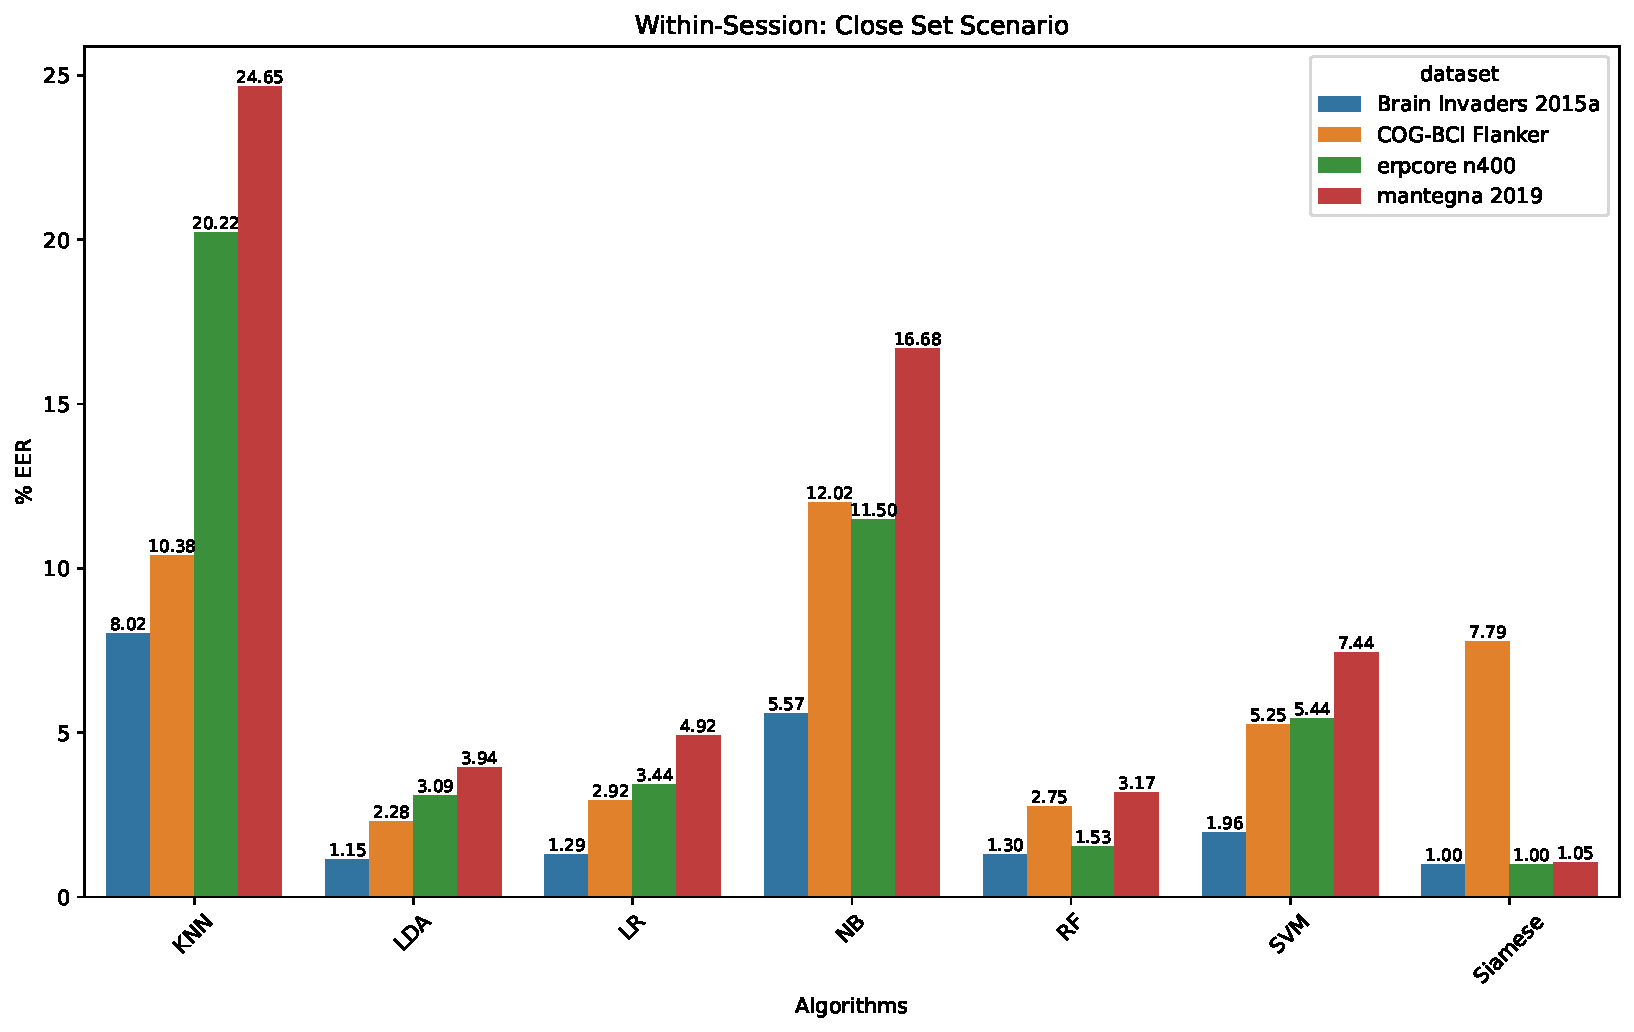
\includegraphics[width=\textwidth]{figures/Results/Within_Session/EER/EER_BAR_Plot_close.pdf}}
    \\
    \subfloat[\centering Mean EER across all subjects in Open-set]{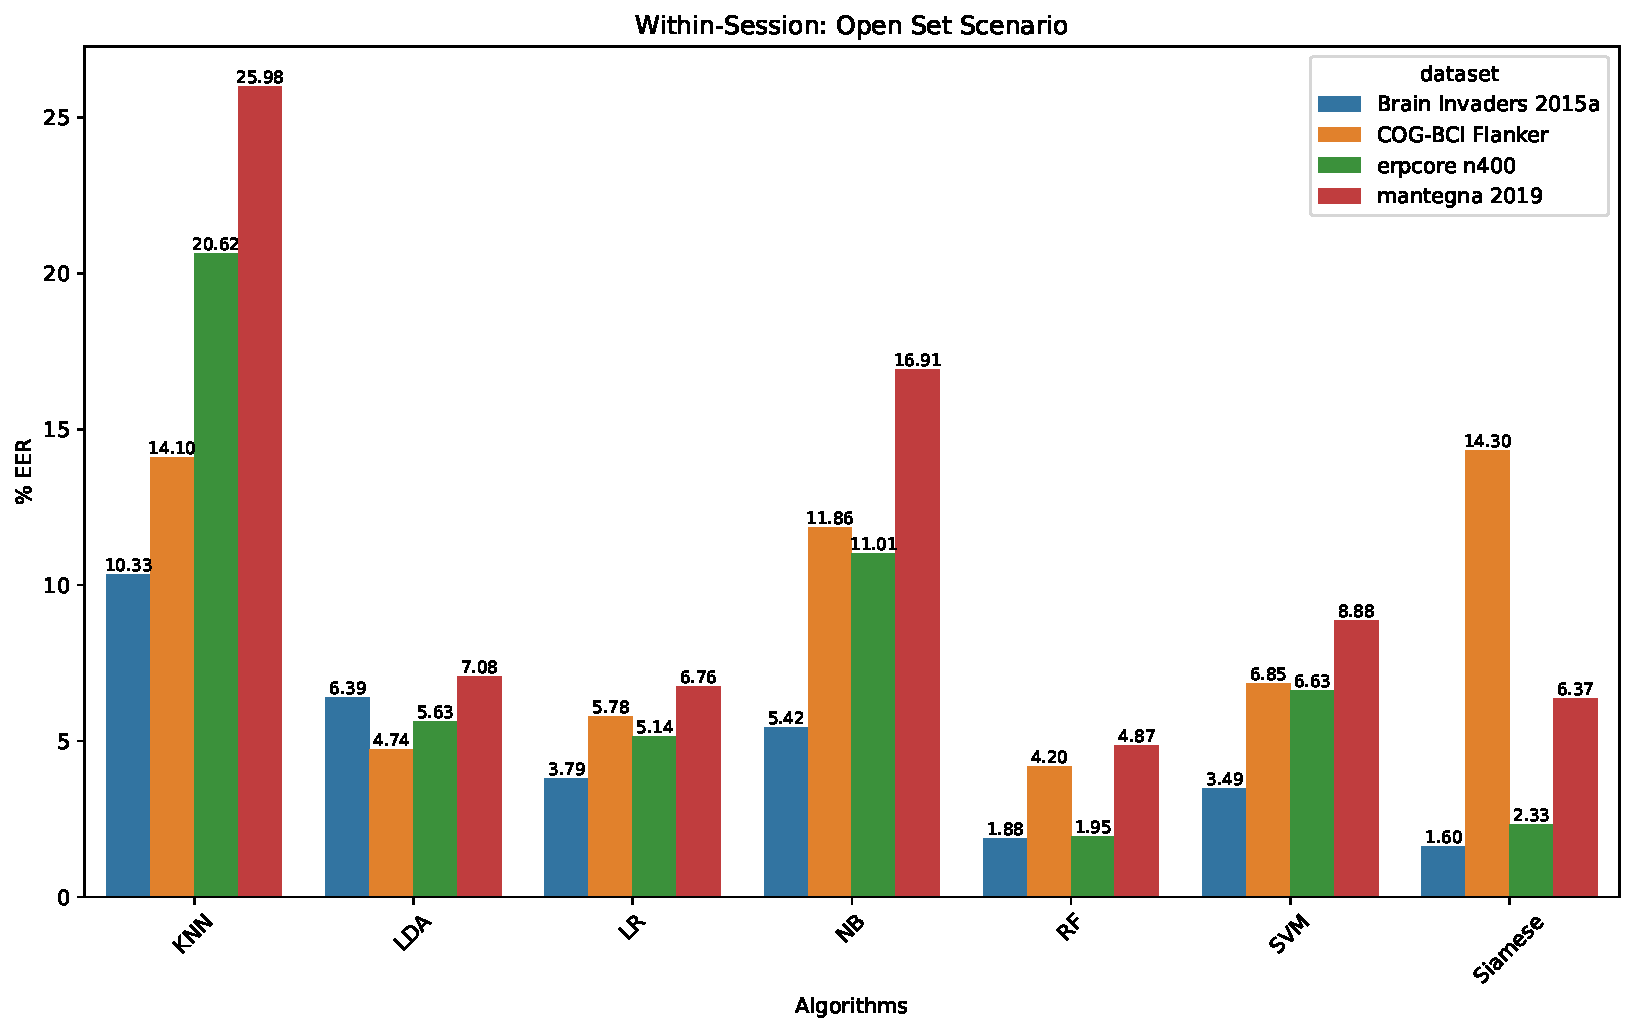
\includegraphics[width=\textwidth]{figures/Results/Within_Session/EER/EER_BAR_Plot_Open.pdf}}
    \caption{Analysis of the four data sets performance using various classifiers and attack scenarios based on mean EER across subjects.}
    \label{fig:WithinSession EER Plots}
\end{figure}

\textbf{\large Comparison between datasets}: BrainInvaders15a performs better than the other datasets, as seen by the data presented in Figure \ref{fig:WithinSession EER Plots}. The achieved EER for BrainInvaders15a demonstrates a notable decrease across all classifiers, except the LDA classifier, when used in the open-set scenario. In this case, the EER of BrainInvaders15a is higher than that of COG-BCI Flanker and ERPCORE: N400. It is worth mentioning that BrainInvaders15a successfully attained an EER of less than 2$\%$ for many classifiers, including LDA, LR, RF, SVM and Siamese in close-set. The superior performance of BrainInvaders15a can also be ascribed to the dataset's larger sample size compared to the other datasets. As mentioned in section \ref{sec:Framework:Pre-Processing}, BrainInvaders15a has 4539 samples as compared to 2193 samples of COG-BCI flanker, 2097 samples of ERPCORE: N400, and 2618 samples of Mantegna2019. The higher number of brain samples allows the increased availability of data, which allows for more robust training of the machine learning model \cite{arias2023performance}. In section \ref{sec:Evaluation:Results:Effect due to different sample size}, we will thoroughly examine the influence of varying brain sample sizes on the performance of classifiers. Furthermore, based on the analysis of the EER in figure \ref{fig:WithinSession EER Plots} and FRR at a FAR of 1$\%$, as presented in Table \ref{tab:Table 3}, it can be observed that the ERPCORE: N400 dataset exhibits the second highest level of performance. This is followed by the COG-BCI flanker dataset and the Mantegna2019 dataset. 
\smallskip

\begin{table}[ht]
\caption{\large{Average FRR at 1$\%$ of FAR for the four datasets in within-session evaluation scheme, comparing different classifiers and  threat case scenarios. The values in the table are shown in percentages.}}

\label{tab:Table 3}
\renewcommand\arraystretch{1.2}
\resizebox{\textwidth}{!}
    {
\begin{tabular}{cc|ccccccc}

\hline

%Table column names
\rule{0pt}{25pt} \textbf{Dataset} & \textbf{Scenario} & \textbf{LDA} & \textbf{SVM} & \textbf{LR} & \textbf{RF} & \textbf{KNN} & \textbf{GNB} & \textbf{Siamese}\\

\hline
% %\rowcolor{Gray}
% \multicolumn{8}{c}{\textbf{\cellcolor{lightgray}Close-Set}} \\
% \hline
% \rule{0pt}{25pt} \textbf{\%EER} & \cellcolor{green}0.767828 & 2.197051 & 1.440007 & 2.164752 & \cellcolor{red}18.8883	\\
\rule{0pt}{25pt} \textbf{BrainInvadeers15a} & \textbf{Close-Set} & 1.04 & 3.61 & 0.98 & 0.89 & 23.46 & 40.54 & 
\textbf{0.05}\\
% \hline
% \multicolumn{8}{c}{\textbf{\cellcolor{lightgray}Open-Set}} \\
% \hline
% \rule{0pt}{25pt} \textbf{\%EER} & 6.440616 & 4.090941 & 5.54588 & \cellcolor{green}2.373961 & \cellcolor{red}21.563637	\\
\rule{0pt}{25pt} \textbf{BrainInvaders15a} & \textbf{Open-Set}& 43.50 & 9.97 & 20.68 & 2.54 & 33.96 & 36.23 & \textbf{2.07}\\
\hline

\rule{0pt}{25pt} \textbf{ERPCORE:N400} & \textbf{Close-Set} & 13.72 & 16.50 & 9.19 & 1.84 & 50.76 & 70.55 & \textbf{0.21}\\
% \hline
% \multicolumn{8}{c}{\textbf{\cellcolor{lightgray}Open-Set}} \\
% \hline
% \rule{0pt}{25pt} \textbf{\%EER} & 6.440616 & 4.090941 & 5.54588 & \cellcolor{green}2.373961 & \cellcolor{red}21.563637	\\
\rule{0pt}{25pt} \textbf{ERPCORE:N400} & \textbf{Open-Set}& 41.25 & 21.90 & 32.02 & \textbf{4.56} & 55.34 & 62.84 & 6.09\\
\hline

\rule{0pt}{25pt} \textbf{Mantegna2019} & \textbf{Close-Set} & 20.52 & 25.90 & 15.85 & 6.89 & 60.99 & 86.13 & \textbf{0.75}\\
% \hline
% \multicolumn{8}{c}{\textbf{\cellcolor{lightgray}Open-Set}} \\
% \hline
% \rule{0pt}{25pt} \textbf{\%EER} & 6.440616 & 4.090941 & 5.54588 & \cellcolor{green}2.373961 & \cellcolor{red}21.563637	\\
\rule{0pt}{25pt} \textbf{Mantegna2019} & \textbf{Open-Set}& 46.51 & 33.43 & 37.38 & \textbf{11.34} & 66.49 & 81.92 & 27.04\\
\hline

\rule{0pt}{25pt} \textbf{COG:BCI Flanker} & \textbf{Close-Set} & 14.05 & 19.19 & 14.05 & \textbf{13.33} & 32.88 & 59.56 & 45.07\\
% \hline
% \multicolumn{8}{c}{\textbf{\cellcolor{lightgray}Open-Set}} \\
% \hline
% \rule{0pt}{25pt} \textbf{\%EER} & 6.440616 & 4.090941 & 5.54588 & \cellcolor{green}2.373961 & \cellcolor{red}21.563637	\\
\rule{0pt}{25pt} \textbf{COG:BCI Flanker} & \textbf{Open-Set}& 28.64 & 19.46 & 28.80 & \textbf{13.87} & 43.25 & 47.17 & 53.60\\
\hline
\end{tabular}
}
\end{table}

\textbf{\large Comparison between close-set and open-set scenarios}: It was hypothesized that the performance of the authentication system would deteriorate when subjected to evaluation in an open-set situation. The findings from our analysis substantiated our initial concerns. As shown in Fig \ref{fig:WithinSession EER Plots}, there is an observed increase in EER ranging from 0.2-5.2$\%$ for most of the classifiers. A similar trend can be seen from table \ref{tab:Table 3} where FRR at $\%$ FAR exhibits an increase ranging from 0.6 to 43.2$\%$. Although almost all the classifiers experience performance degradation when comparing their results in close-set and open-set settings, the most significantly impacted classifiers are LDA and LR. A notable performance decline is observed for classifier LDA where EER for dataset BrainInvaders15a increased from mere 1.13$\%$ in closed-set to 6.3$\%$ in open-set, a significant 6-fold increase. 
\smallskip

The outcomes of the close-set and open-set may be influenced by the differing sizes of the spaces occupied by the potential attackers in each scenario \cite{arias2023performance}. As outlined in section \ref{sec:Framework:Classification:Supervised based Learning Classification}, the evaluation strategy of close-set requires training the authentication model with N-1 attackers where N represents the total number of users. In contrast, the classifiers in an open-set scenario learn from approximately three-quarters of the N-1 attackers. Consequently, in close-set settings, the attacker spaces are more significant than in open-set, thereby enabling more effective training of machine learning models in close-set. Additionally, in close-set environments, the system is designed to optimize its ability to discern a particular group of pre-identified users(enrolled users). This approach produces favorable results due to the limited variability in the training set. However, in the context of open-set scenarios, the model is required to effectively address the existence of unseen users, which introduces the additional complexity of accurately identifying authorized and unauthorized users. 
\smallskip

\begin{figure}[htbp]
    \centering
    
    \begin{minipage}{0.42\textwidth}
        \centering
        \subfloat[ROC: BrainInvaders15a Close-Set]{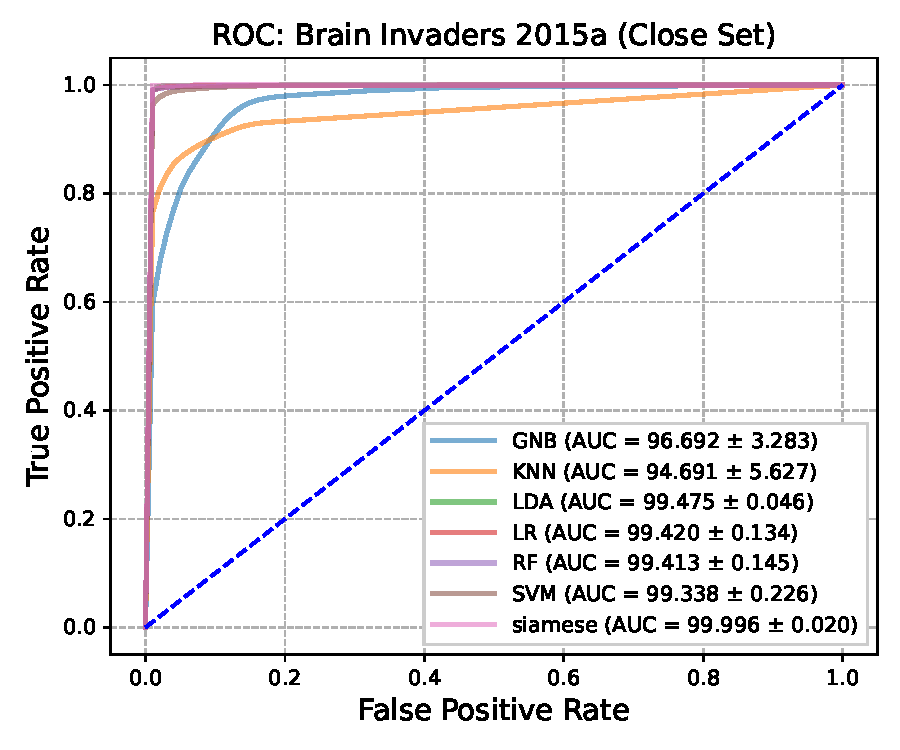
\includegraphics[width=0.9\textwidth]{figures/Results/Within_Session/ROC/ROC Brain Close.pdf}}
        
        \subfloat[ROC: ERPCORE N400 Close-Set]{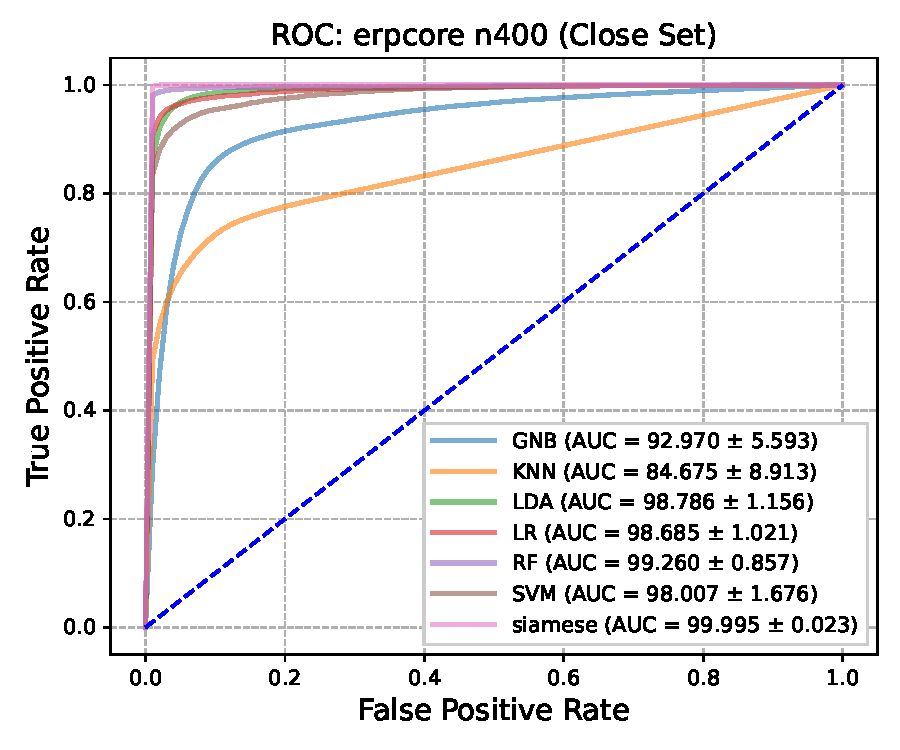
\includegraphics[width=0.9\textwidth]{figures/Results/Within_Session/ROC/ROC ERPCORE Close.pdf}}
        
        \subfloat[ROC: Mantegna 2019 Close-Set]{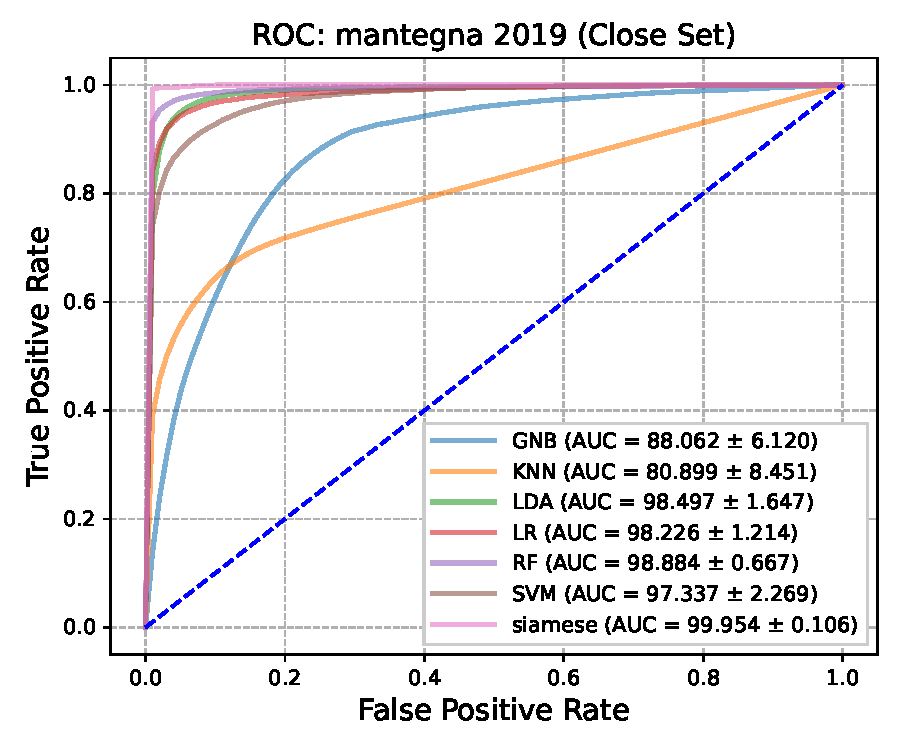
\includegraphics[width=0.9\textwidth]{figures/Results/Within_Session/ROC/ROC Mantegna Close.pdf}}
        
        \subfloat[ROC: COGBCI Flanker Close-Set]{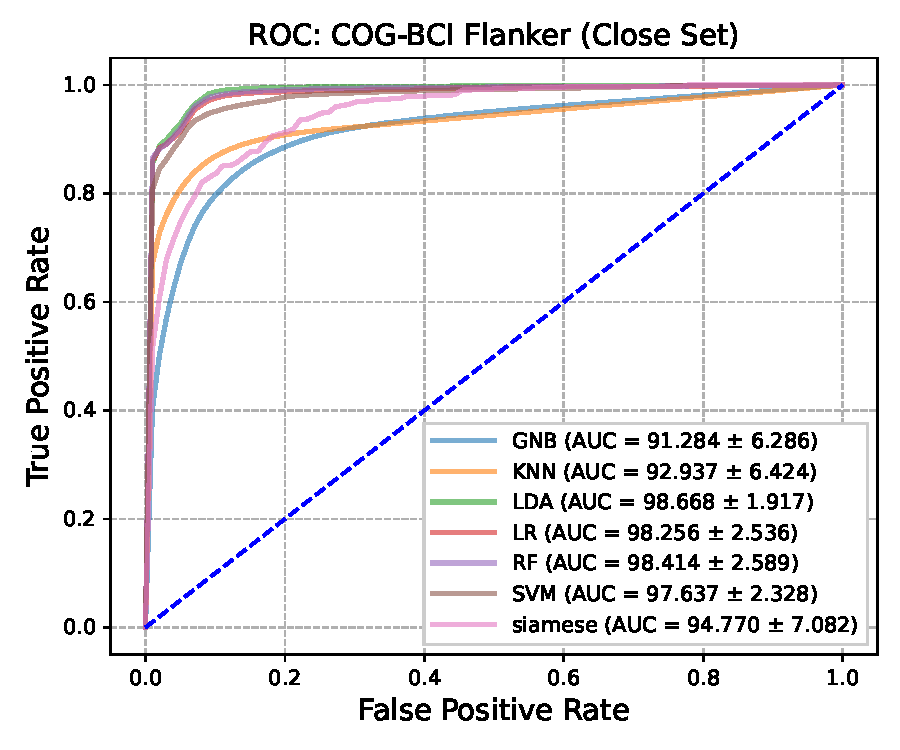
\includegraphics[width=0.9\textwidth]{figures/Results/Within_Session/ROC/ROC COG Close.pdf}}
    \end{minipage}%
    \begin{minipage}{0.42\textwidth}
        \centering
        \subfloat[ROC: BrainInvaders15a Open-Set]{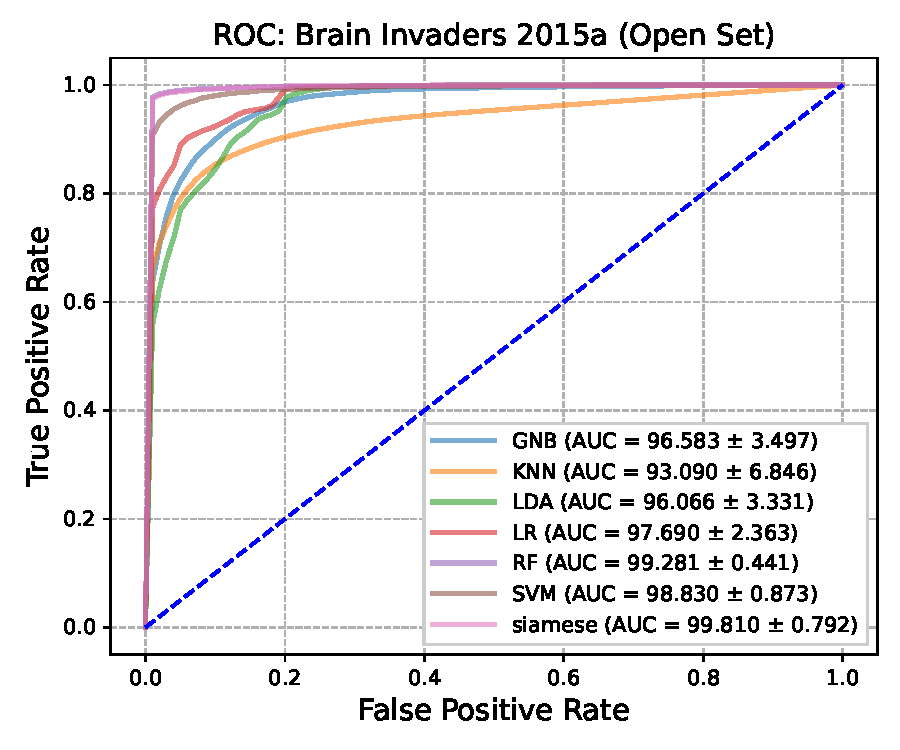
\includegraphics[width=0.9\textwidth]{figures/Results/Within_Session/ROC/ROC Brain Open.pdf}}
        
        \subfloat[ROC: ERPCORE N400 Open-Set]{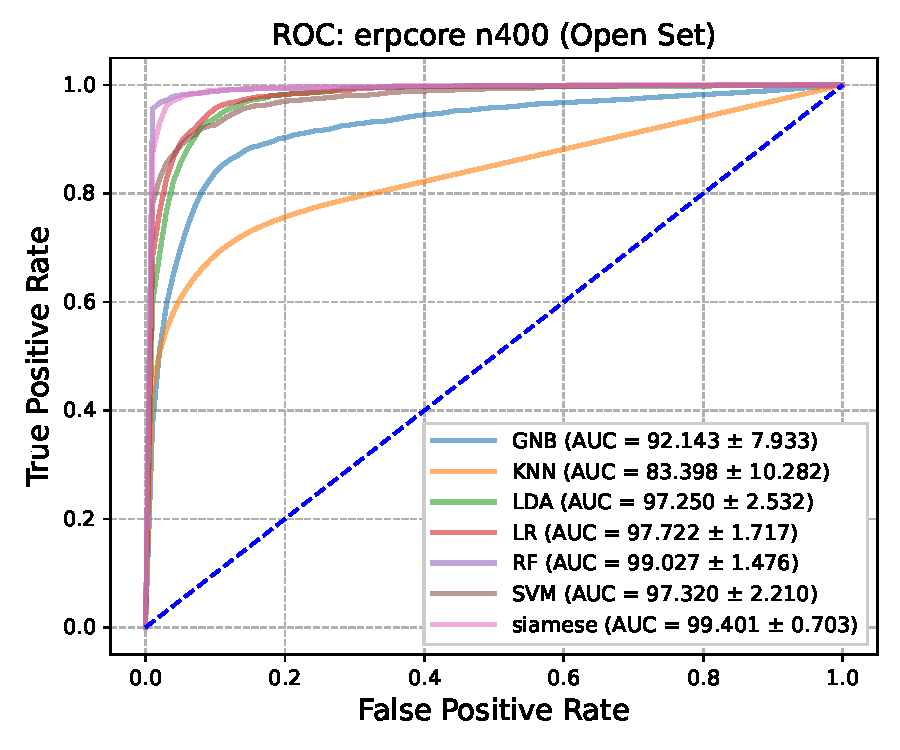
\includegraphics[width=0.9\textwidth]{figures/Results/Within_Session/ROC/ROC ERPCORE Open.pdf}}
        
        \subfloat[ROC: Mantegna 2019 Open-Set]{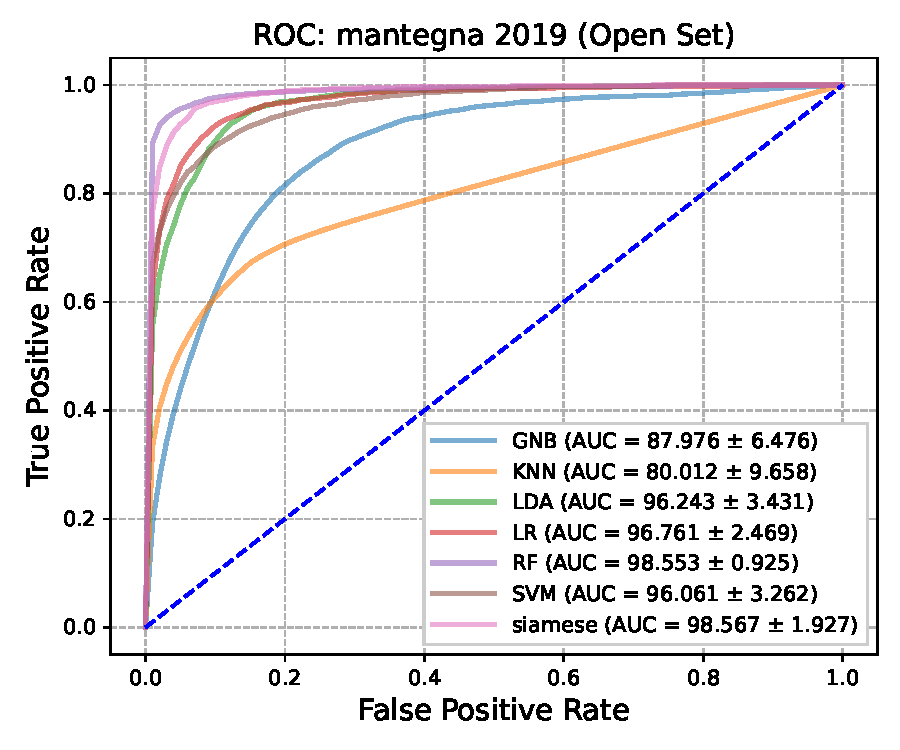
\includegraphics[width=0.9\textwidth]{figures/Results/Within_Session/ROC/ROC Mantegna Open.pdf}}
        
        \subfloat[ROC: COGBCI Flanker Open-Set]{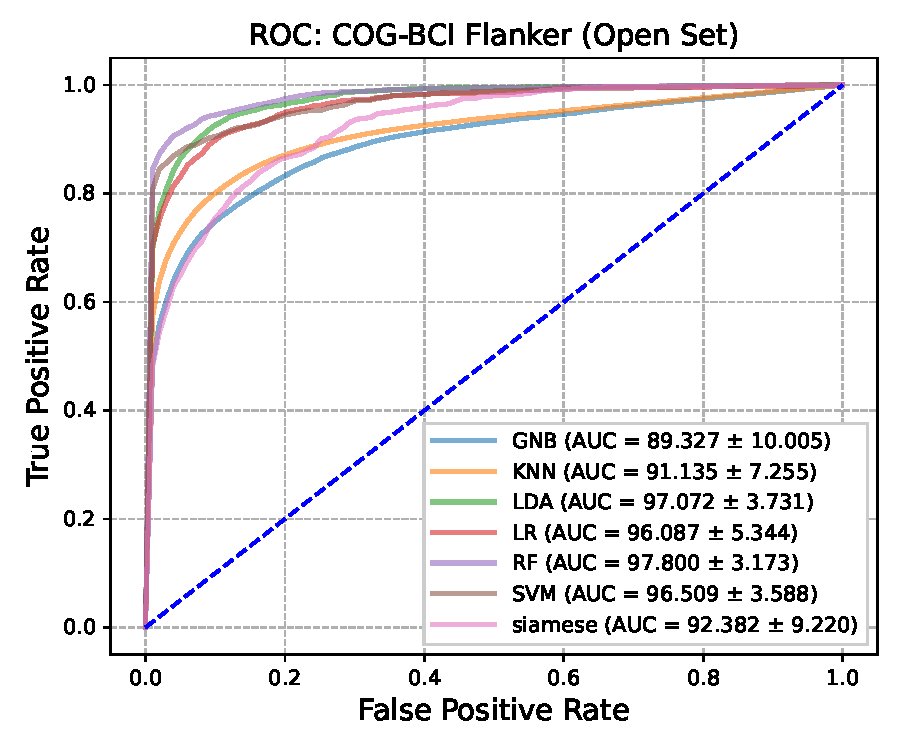
\includegraphics[width=0.9\textwidth]{figures/Results/Within_Session/ROC/ROC COG Open.pdf}}
    \end{minipage}
    
    \caption{Comparative analysis of ROC-Curves for all 4 datasets in within-session evaluation}
    \label{fig:WithinSession ROC Curve}
\end{figure}

\textbf{\large Comparison between traditional and deep learning methods}: 
Traditional machine learning algorithms such as LDA, SVM, LR, RF, KNN, and GNB have always been widely utilized in EEG-based authentication systems. These algorithms provide good results when the number of classes is known and fixed. However, the performance of these algorithms tends to decline when they are tested with smaller data samples. They also necessitate extracting discriminant features from the raw EEG data. To address these problems, researchers started focusing on deep learning methods such as Siamese Networks, which learn directly from the time series EEG data, removing the overhead of the feature extraction process. Moreover, they do not require retraining while adding new users to the system. As a result, Siamese networks have achieved remarkable success in biometrics-based authentication studies such as face recognition \cite{wu2017face, facenet, heidari2020using} and Brainwave authentication \cite{fallahi2023brainnet, maiorana2019eeg}. 
\smallskip

The results obtained in our study have also demonstrated Siamese networks as the best-performing algorithm among all the traditional classifiers. The ROC-Curves of the four datasets are presented in Figure \ref{fig:WithinSession ROC Curve}, showcasing the operational capabilities of the traditional and deep learning authentication models in closed-set and open-set settings. The Area Under Curve (AUC) under ROC-Curve represents a single value representing the system's ability to differentiate between genuine users and imposters \cite{arias2023performance}. A higher AUC implies an improved performance as it indicates the system has a higher True Positive Rate (TPR) value and a lower False Positive Rate (FPR). The Siamese Networks have a higher AUC score than traditional classifiers in close-set and open-set scenarios across most datasets. However, it is worth noting that in the COG-BCI flanker dataset, classifiers like LDA, LR, SVM and RF outperforms the Siamese Networks regarding the AUC score for both threat cases. The findings depicted in Figure \ref{fig:WithinSession EER Plots} EER Plots regarding the average EER align with the earlier observation. The results indicate that Siamese networks are superior to other classifiers in attaining EERs for the BrainInvaders15a, ERPCORE: N400, and Mantegna2019 datasets. 
\smallskip

%We have also calculated the standard deviation in AUC among the classifiers for each dataset. We observed that there is a high variability among the traditional classifiers, especially GNB and KNN. On the other hand, Siamese networks has very less variability for datasets BrainInvaders15a, ERPCORE: N400, and Mantegna2019. However, the calculated standard deviation for Siamese Networks in COG-BCI Flanker dataset is as high as 9.2. 
%The considerable variability observed in the COG-BCI Flanker dataset can be explained by implementing epoch rejection during the pre-processing stage, as discussed in section \ref{sec:Framework:Pre-Processing}. This process resulted in a disparity where specific individuals had a limited number of samples while others had ample samples. Consequently, significant variation was seen among the samples across the subjects.  
%
%\smallskip 
\textbf{\large Usability}: FAR is a crucial metric when assessing the overall security of the authentication system because it represents how many times the system allows an unauthorized user to authenticate. Therefore, the FAR threshold for most authentication systems is generally set low. The FAR's relevance spans across a spectrum, with a lower threshold of 1$\%$ for applications with lower security requirements and an even more stringent point of 0.00001$\%$ for applications necessitating the highest levels of security \cite{ann2007biometric}. On the hand, FRR quantifies the effectiveness of the authentication system in terms of its usability. A low FRR indicates that authentic users are not experiencing rejections. It is essential to strike a balance between the two metrics as each increase at the expense of the other. Consequently, we calculated FRR and FAR at 1$\%$ for each dataset in close-set and open-set. By assessing the system's performance at this particular threshold of FAR and FRR, we can gain insights into the system's efficacy in real-world situations. For example, a higher value of FRR at 1$\%$ FAR implies that genuine users are being denied access more frequently, hence adversely affecting the overall user experience. Conversely, a low FRR and FAR of 1$\%$ indicate that the system effectively identifies and accepts genuine users while upholding an acceptable level of security. 
\smallskip

The findings presented in Table \ref{tab:Table 3} indicate that the most optimal setup is achieved when employing Siamese Networks on dataset BrainInvaders15a for authentication. Remarkably, the closed-set scenario achieves FRR of just 0.05$\%$ at threshold of 1$\%$ FAR. 
%In the context of the open-set scenario, a value of 2.527$\%$ is attained. 
The authentication system demonstrates high usability and resilience in open-set situations, as seen by a FRR value of only 2.07$\%$. This suggests that the system remains effective even when faced with previously unseen attackers. RF has demonstrated its effectiveness as the second-highest-performing classifier in multiple instances. Specifically, it achieved the best FRR at a FAR of 1$\%$ in four different scenarios: ERPCORE: N400 (open-set), Mantegna2019 (open-set), and COG-BCI Flanker (close and open-set). 

%is the second best classifier as it attained best FRR at 1$\%$ FAR on four occasions such as ERPCORE: N400 (open-set), Mantegna2019(open-set) and COG-BCI Flanker (close and open-set). 
%In the open-set scenario, value of 2.527$\%$ is achieved. A FRR value value of mere 2.527$\%$ in open-set settings indicates the high usability and robustness of our authentication system even when it is exposed to unseen attackers. It can also be seen that    
%we achieve FRR at 1$\%$ FAR 0.059$\%$ in close-set and 2.527$\%$ in open-set. 

\subsection{Cross-Session Evaluation Results}
\label{sec:Evaluation:Results:Cross-Session Evaluation results}
This section focuses on the outcomes derived from conducting evaluations throughout multiple sessions. The cross-session review is run solely on the COG-BCI Flanker dataset, which represents the only dataset available. Figure \ref{fig: Cross_session_EER_Close_set} and \ref{fig: Cross_session_ROC_Close_set} illustrate the outcomes of all classifiers applied to COG-BCI Flanker in terms of the mean EER and ROC-Curve, as determined by the cross-session evaluation. The performance of all the classifiers in both the close-set and open-set scenarios was observed to be comparable in cross-session. Therefore, the findings shown in both figures pertain to the close-set scenario. As depicted in Figure \ref{fig: Cross_session_EER_Close_set}, %Siamese Network has the least EER among all the classifiers. 
The attained EER for the traditional classifiers, namely LR and LDA is identical. Both classifiers have also achieved the least EER among all the classifiers. However, LR demonstrates superior performance compared to LDA when evaluating its performance based on the AUC metric. This can be observed in \ref{fig: Cross_session_ROC_Close_set}, where the Receiver Operating Characteristic (ROC) curves indicate that LR has attained a slightly higher AUC value. The Siamese Network demonstrates the third highest classification performance, achieving an EER of 19.3$\%$. Although RF exhibited outstanding performance in within-session evaluation, surpassing all classical classifiers and Siamese Networks, its performance in cross-session evaluation is unsatisfactory. RF is the fourth best-performing classifier, exhibiting a notable EER of 26.9$\%$. Additionally, the results of the cross-session evaluation support the conclusions drawn from the within-session evaluation, indicating that the GNB and KNN classifiers demonstrate the highest EER values compared to other classifiers.  
%Similar to within-session evaluation, GNB and KNN have the highest EER among all the classifiers. 
This finding suggests the need for additional exploration into these two classifiers limitations and possible enhancements. 
\begin{figure*}
    %
    \centering
     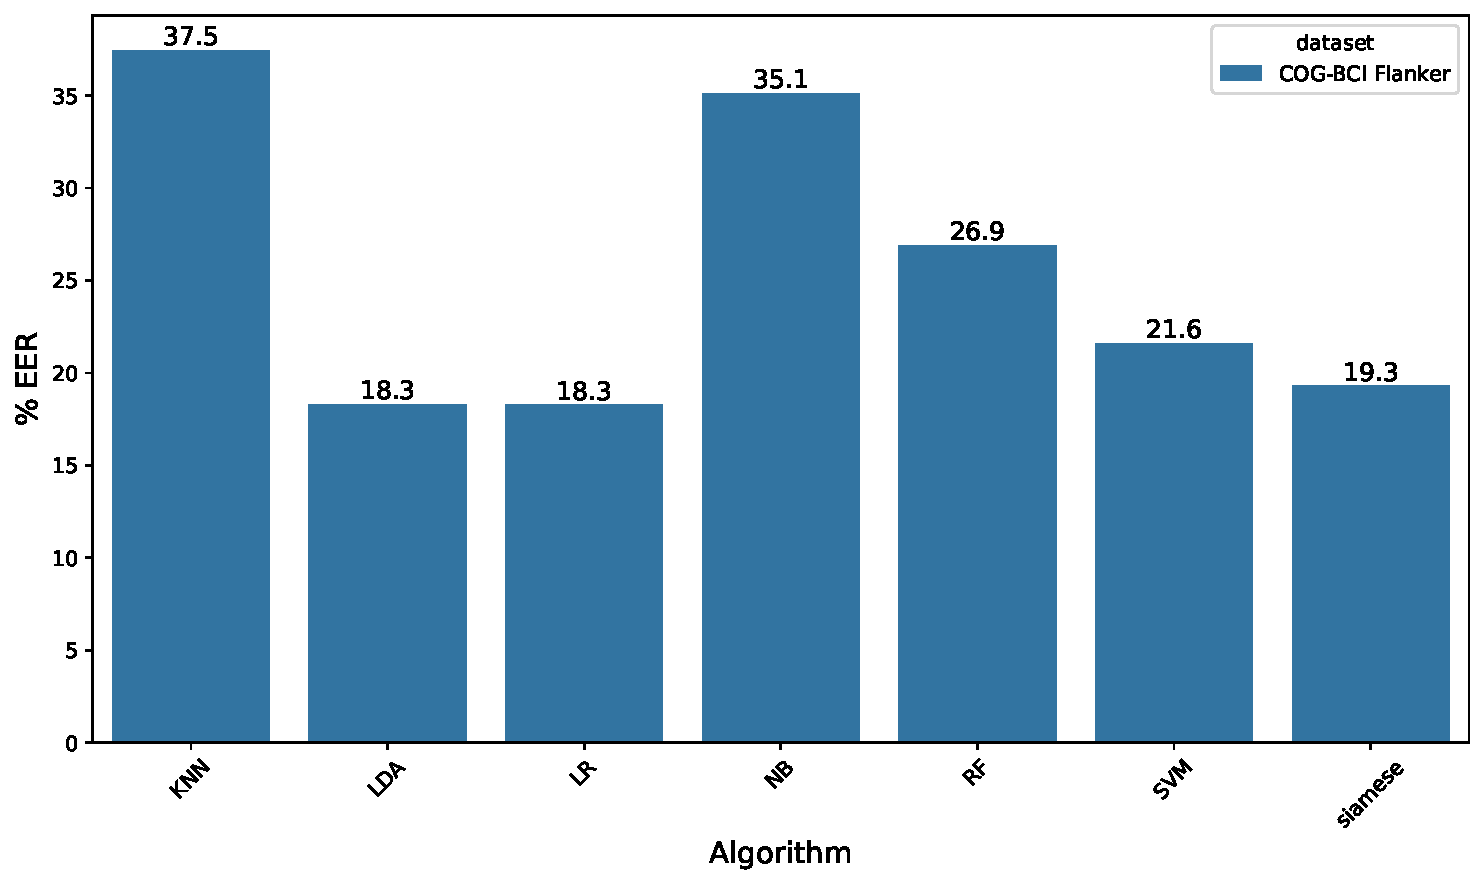
\includegraphics[width=0.85\textwidth]{figures/Results/Cross_Session/EER/EER_plot_close_Set.pdf}  
    %
    
    %\caption{SMC Learning Algorithm}
    \caption{Average EER for cross-session evaluation on COG-BCI Flanker dataset, comparing performance across different authentication algorithms}
    \label{fig: Cross_session_EER_Close_set}
\end{figure*}

\begin{figure*}
    %
    \centering
     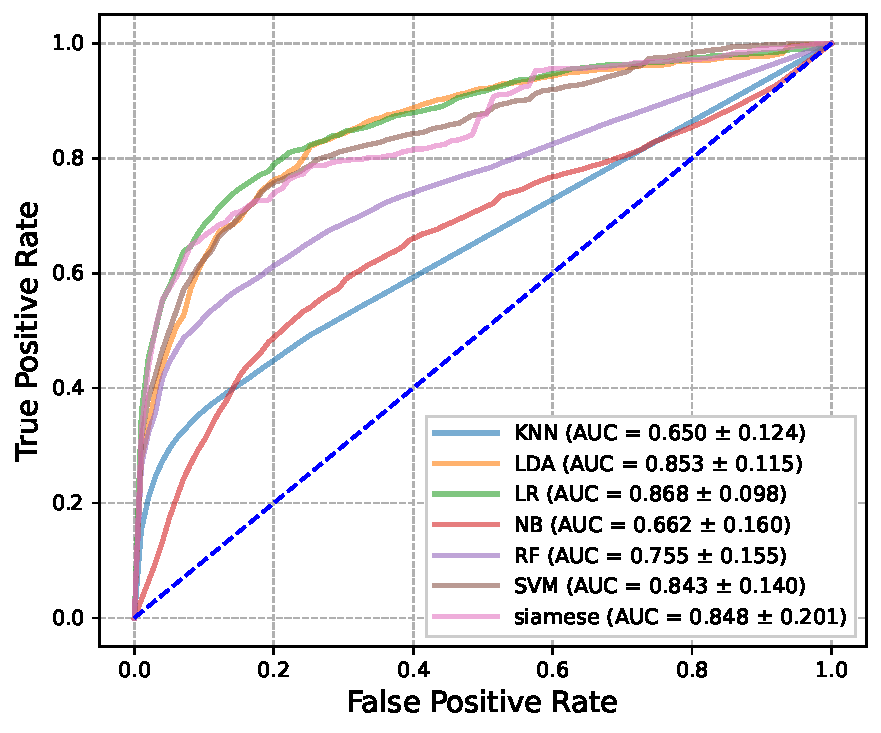
\includegraphics[width=0.75\textwidth]{figures/Results/Cross_Session/ROC_CURVE/ROC_Curve_Close_set_cross_session.pdf}  
    %
    
    %\caption{SMC Learning Algorithm}
    \caption{Performance comparison of the dataset COG-BCI Flanker in cross-session evaluation scheme. ROC Curves are depicted for different classifiers in close-set attacker scenario.}
    \label{fig: Cross_session_ROC_Close_set}
\end{figure*}

The findings from the cross-session evaluation conducted on the COG-BCI Flanker dataset have provided valuable insights into noteworthy observations. We did not achieve the best possible results in cross-session. One possible explanation for the sub-optimal performance in cross-session evaluation is the increased variability and unpredictability due to the time duration between the enrollment and authentication process. As mentioned in section \ref{sec:Framework:Classification:Similarity Based Learning} and \ref{sec:Framework:Classification:Supervised based Learning Classification}, we performed enrollment for each subject by utilizing the brain sample acquired in two sessions and performed authentication on the remaining session's EEG data.
This temporal gap may have resulted in changes to the EEG signals, making it challenging for the classifiers to recognize users consistently across sessions. The other factors which could impact the results in cross-session settings are the electrode resetting across the sessions, variations in human brain states, and template ageing \cite{seha2020eeg}. Moreover, the performance of traditional algorithms appears to have been impact more prominently in cross-session evaluation than Siamese Networks.  
\smallskip

The results of our cross-session setting align with Arnau-González \textit{et al.} \cite{arnau2018influence} work, which utilized three publicly available datasets to investigate user identification in both single-session and multi-session scenarios. Similar to our study, Arnau-González et al. also performed feature extraction by computing Power Spectral Density across Theta, Delta, Alpha, Beta, and Gamma bands and utilized classifiers such as SVM, KNN, Multilayer Perceptron (MLP), and AdaBoost for building the identification models. The researchers opted to use accuracy as the performance metric in their investigation. The classifiers exhibited much-improved performance in the single session setup, with accuracy rates over 90$\%$ for various classifiers across all datasets. Nevertheless, the system's performance showed a notable decline during the evaluation conducted under a cross-session scenario. The accuracy reached in cross-session evaluation was 79$\%$, a substantial decrease compared to the accuracy of 99$\%$ gained in single-session evaluation. The consistent findings between our cross-session study and the work of Arnau-González et al. emphasize the need to consider temporal factors when creating authentication models for practical deployment.     

%Accuracy was chosen as the performance metric in their study. The performance of most of the classifiers was significantly better in single session setup where achieved accuracy was more than 90$\%$ for various classifiers in each dataset. However, the performance was considerably low when the system was evaluated under cross-session scenario. In cross-session, the best achieved accuracy was 79$\%$, a significant drop from the best achieved accuracy of 99$\%$ in single-session evaluation.     

%three publicly available
%datasets, one of which consisted of EEG data obtained over three distinct sessions, while the remaining dataset contained EEG data from a single session.   
%multi-session datasets such as DEAP \cite{koelstra2011deap}, MAHNOB-HCI \cite{soleymani2011multimodal} and SEED \cite{zheng2015investigating} for evaluating the EEG variability across sessions.       

\subsection{Within-Session Vs Cross-Session}
One of the main objectives of this thesis is to comprehensively study the impact of EEG variability across single and multi-session settings. We conducted thorough evaluations of our authentication models in both within-session and cross-session scenarios, as detailed in the preceding sections, and the results are presented in sections \ref{sec:Evaluation:Results:Within-Session Evaluation Results} and \ref{sec:Evaluation:Results:Cross-Session Evaluation results} respectively. These evaluations have yielded significant insights into the performance of our classifiers in different conditions and have illuminated the difficulties associated with temporal variations in EEG signals. 
In this section, we will compare the results obtained from both the within-session and cross-session evaluation schemes. According to Table 4\ref{tab:Table 4}, the results of the multi-session (cross-session) evaluation are significantly poorer than single-session (within-session) evaluation for dataset COG-BCI Flanker. A significant decrease in the performance of RF can be observed, which was identified as the most efficient classifier across all datasets for within-session evaluation, as discussed in section \ref{sec:Evaluation:Results:Within-Session Evaluation Results}. The cross-session EER experiences a substantial increase of 878.5$\%$ (from 2.75$\%$ to 26.91$\%$) and FRR at 1$\%$ FAR raises to 450.8$\%$ (from 13.33$\%$ to 73.43$\%$). LR and LDA which have comparable EER and FRR at 1$\%$ FAR in within-session also experiences performance degradation as EER increases from 2.28$\%$ to 18.32$\%$ for LDA and 2.92$\%$ to 18.28$\%$ for LR. Furthermore, the Siamese Networks likewise exhibit an increase trend in EER. However, the rise in the EER was only 147.7 (from 7.79$\%$ to 19.30$\%$), indicating that the observed decline in performance was less pronounced in Siamese Networks compared to traditional classifiers.
\smallskip

The Siamese Networks, a deep learning technique, exhibited a higher level of resilience in both within-session and cross-session evaluations, which is a favorable finding. Although the Siamese Networks also showed an elevation in EER, the magnitude of this increase was noticeably less significant compared to traditional classifiers. The observation as mentioned above implies that Siamese Networks has the ability to learn underlying feature representations  and capture similarities among EEG samples, hence exhibiting enhanced resilience to temporal variations in EEG signals. The efficacy of Siamese Networks in addressing cross-session evaluations underscores the potential of deep learning techniques in mitigating some constraints encountered by traditional classifiers, thereby presenting encouraging prospects for further investigation in EEG-based authentication systems.



 
% \begin{figure*}
%     %
%     \centering
%      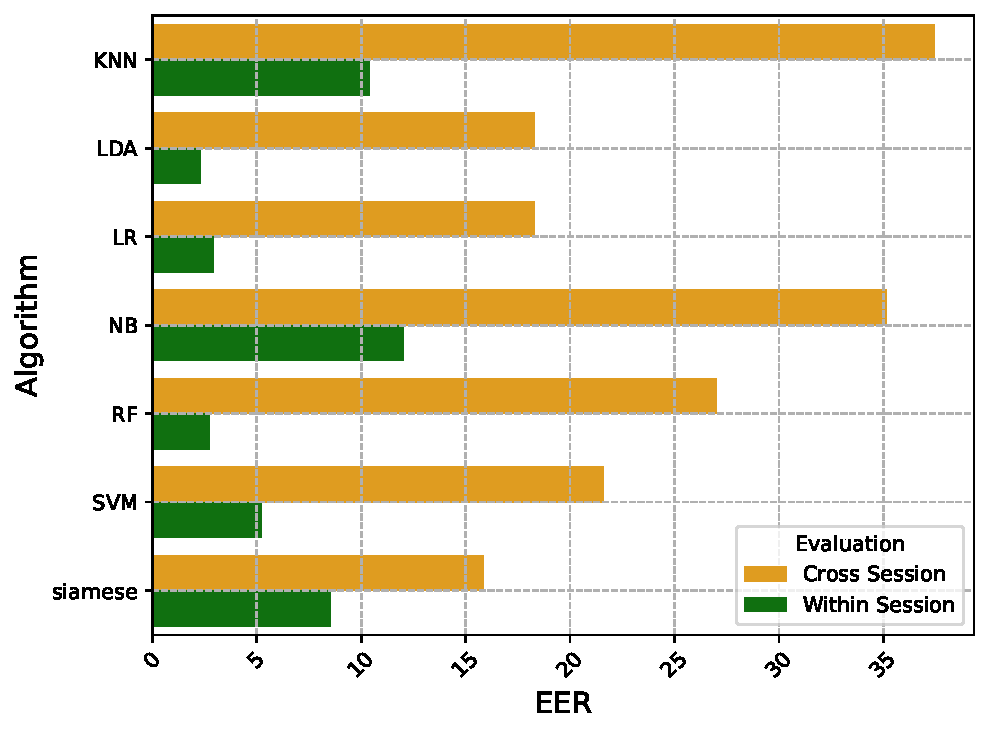
\includegraphics[width=0.75\textwidth]{figures/Results/Within Vs Cross/WithinSession_vs_CrossSession_close_set.pdf}  
%     %
    
%     %\caption{SMC Learning Algorithm}
%     \caption{EER values of the proposed system in the cross-session configuration versus the within-session configuration.}
%     \label{fig: EER_within_vs_cross}
% \end{figure*}

\begin{table}[ht]
\caption{\large{Average Performance of classifiers on the COG-BCI Flanker \cite{cogbci} dataset, comparing Within-Session and Cross-Session Evaluation}}

\label{tab:Table 4}
\renewcommand\arraystretch{1.2}
\resizebox{\textwidth}{!}
    {
\begin{tabular}{c|ccccccc}

\hline

%Table column names
\rule{0pt}{25pt} \textbf{Metric} & \textbf{LDA} & \textbf{SVM} & \textbf{LR} & \textbf{RF} & \textbf{KNN} & \textbf{GNB} & \textbf{Siamese}\\

\hline
%\rowcolor{Gray}
\multicolumn{8}{c}{\textbf{\cellcolor{lightgray}Within-Session}} \\
\hline
\rule{0pt}{25pt} \textbf{\%EER} & $2.28 \pm 2.55$ & $5.25 \pm 3.50$ & $2.92 \pm 3.28$ & $2.75 \pm 3.28$ & $10.38 \pm 6.92$ & $12.02 \pm 7.24$ & $7.79 \pm 6.54$	\\
\rule{0pt}{25pt} \textbf{FRR at 1$\%$ FAR} & 14.46 & 19.19 & 14.05 & 13.33 & 32.88 & 59.56 & 45.07 \\
\hline
\multicolumn{8}{c}{\textbf{\cellcolor{lightgray}Cross-Session}} \\
\hline
\rule{0pt}{25pt} \textbf{\%EER} & $18.32 \pm 11.47$ & $21.58 \pm 13.18$ & $18.28 \pm 11.47$ & $26.91 \pm 13.67$ & $37.47 \pm 10.34$ & $35.15 \pm 13.80$ & $19.30 \pm 17.49$	\\
\rule{0pt}{25pt} \textbf{FRR at 1$\%$ FAR} & 72.37 & 68.74 & 64.15 & 73.43 & 84.66 & 96.83 & 67.53 \\
\hline
\end{tabular}
}
\end{table}

%%%%%%%%%%%%%%%%%%%%%%%%%%%%%%%%%%%%%%%%%%%%%%%%%%%%%%%%%%%%%%%%%%%%%
%%%%%%%%%%%%%%%%%%%%%%%%% AR Features %%%%%%%%%%%%%%%%%%%%%%%%%%%%%%%
%%%%%%%%%%%%%%%%%%%%%%%%%%%%%%%%%%%%%%%%%%%%%%%%%%%%%%%%%%%%%%%%%%%%%

\begin{figure}%
    \centering
    \subfloat[\centering  Effect of AR features with orders (1 to 10) on performance of the dataset BrainInvaders15a]{{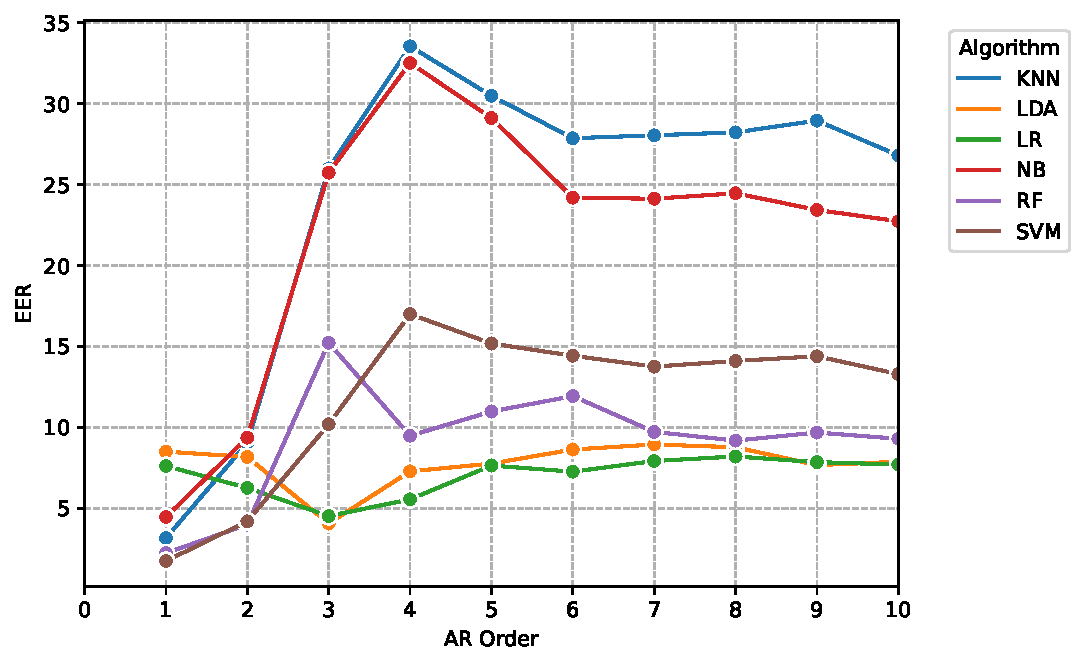
\includegraphics[width=7.6cm]{figures/Results/Other_Plots/Feature_Extraction/BrainInvaders/Brain_AR.pdf}}}%
    \qquad
    \subfloat[\centering Effect of AR features with orders (1 to 10) on performance of the dataset COGBCI Flanker]{{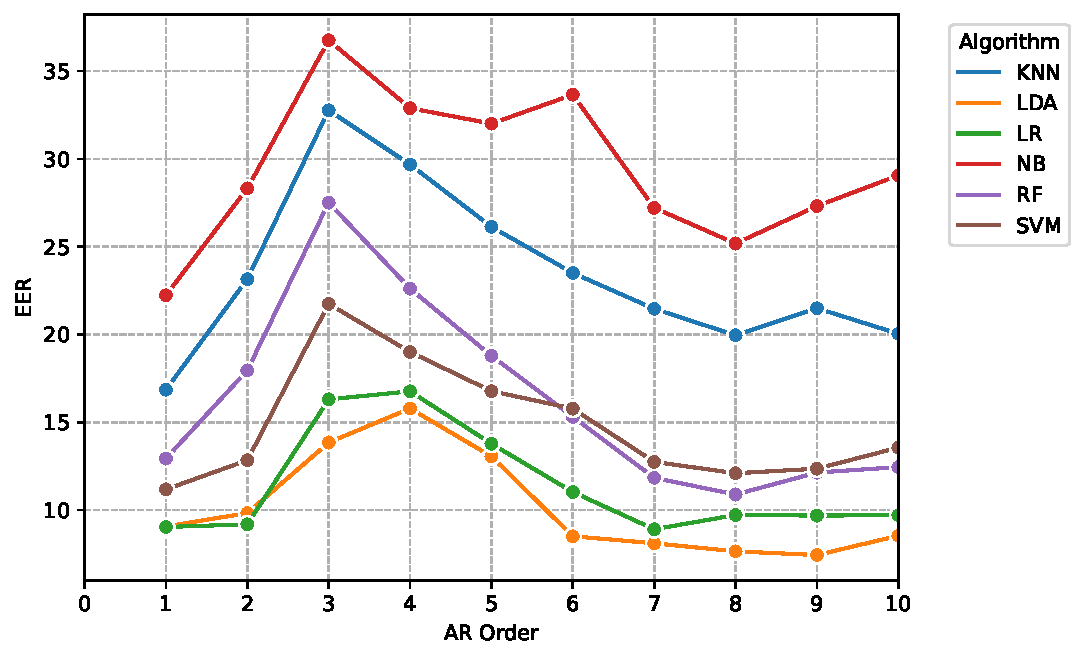
\includegraphics[width=7.6cm]{figures/Results/Other_Plots/Feature_Extraction/COGBCI/cog_AR.pdf}}}%
    % \caption{Impact of Auto Regressive(AR) Features with orders from 1 to 10 on the performance of the dataset.}%
    
    \subfloat[\centering Effect of AR features with orders (1 to 10) on performance of the dataset ERPCORE: N400]{{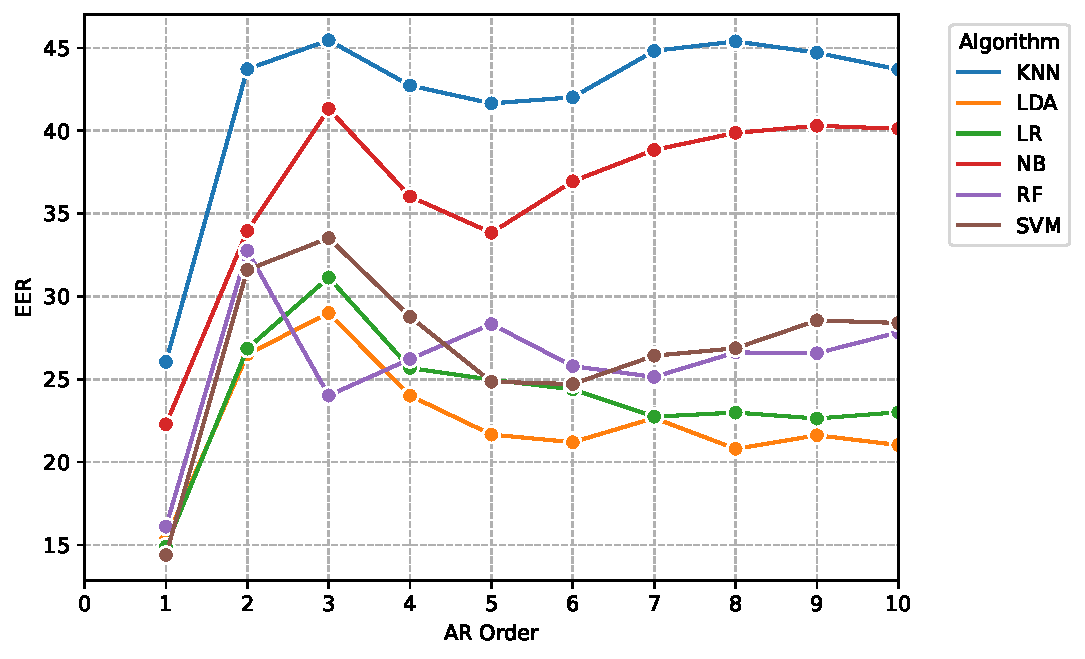
\includegraphics[width=7.6cm]{figures/Results/Other_Plots/Feature_Extraction/ERPCORE/ERPCORE_AR.pdf}}}%
    \qquad
    \subfloat[\centering Effect of AR features with orders (1 to 10) on performance of the dataset Mantegna2019]{{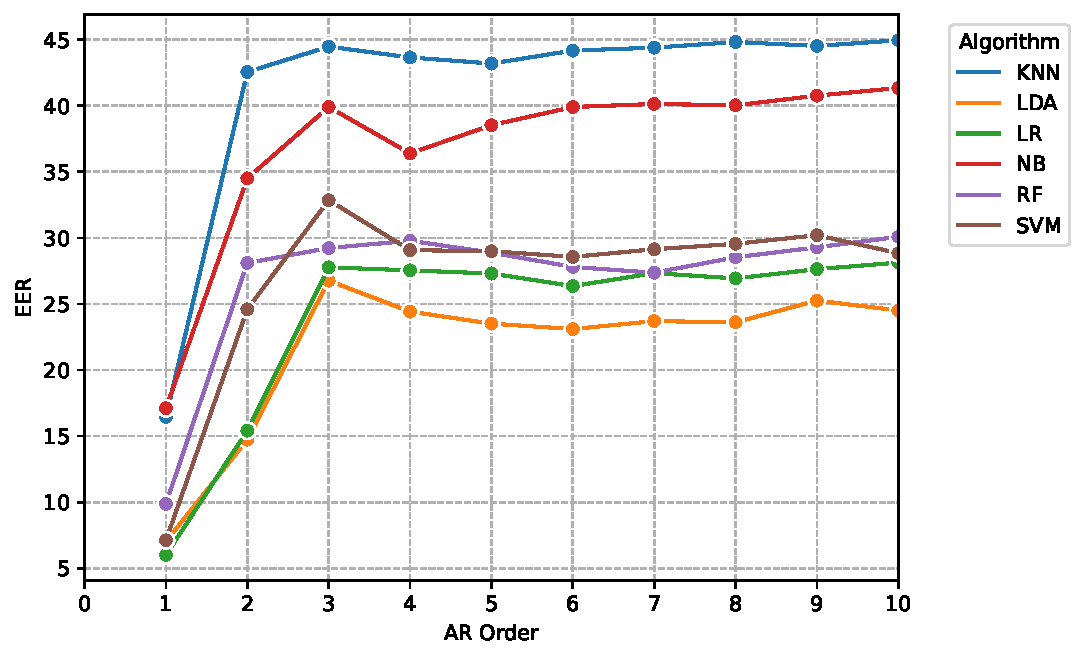
\includegraphics[width=7.6cm]{figures/Results/Other_Plots/Feature_Extraction/MANTEGNA/MANTEGNA_AR.pdf}}}%
    \caption{Impact of Auto Regressive(AR) Features on the performance of the datasets. Figures (a), (b), (c) and (d) depicts the change in the EER of the traditional classifiers for the datasets BrainInvaders51a, COG-BCI Flanker, ERPCORE: N400 and Mantegna2019 respectively. }%
    \label{fig: Feature Extraction using AR}%
\end{figure}

%%%%%%%%%%%%%%%%%%%%%%%%%%%%%%%%%%%%%%%%%%%%%%%%%%%%%%%%%%%%%%%%%%%%%
%%%%%%%%%%%%%%%%%%%%%%%%% PSD Features %%%%%%%%%%%%%%%%%%%%%%%%%%%%%%
%%%%%%%%%%%%%%%%%%%%%%%%%%%%%%%%%%%%%%%%%%%%%%%%%%%%%%%%%%%%%%%%%%%%%
\begin{figure}%
    \centering
    \subfloat[\centering Effect of PSD features on the performance of the dataset BrainInvaders15a]{{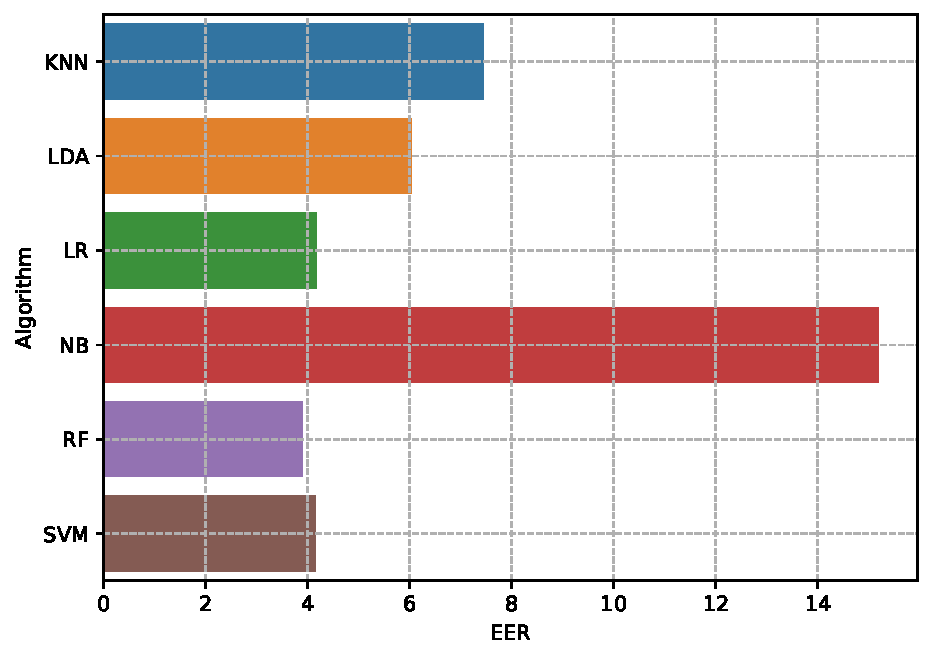
\includegraphics[width=7.60cm]{figures/Results/Other_Plots/Feature_Extraction/BrainInvaders/Brain_PSD.pdf}}}%
    \qquad
    \subfloat[\centering Effect of PSD features on the performance of the dataset COG-BCI Flanker]{{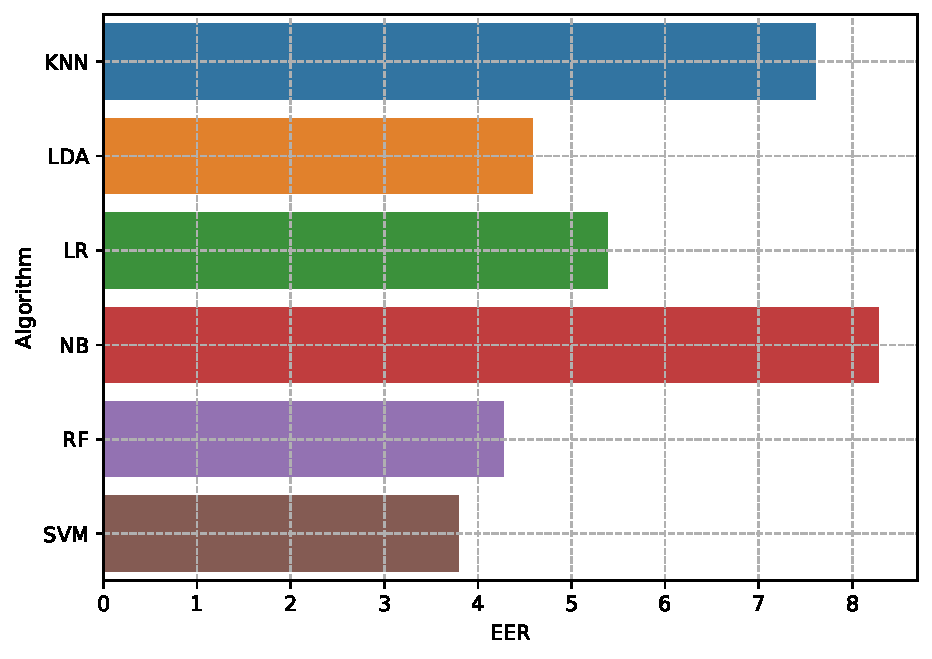
\includegraphics[width=7.6cm]{figures/Results/Other_Plots/Feature_Extraction/COGBCI/cog_PSD.pdf}}}%
   
    \subfloat[\centering Effect of PSD features on the performance of the dataset ERPCORE: N400]{{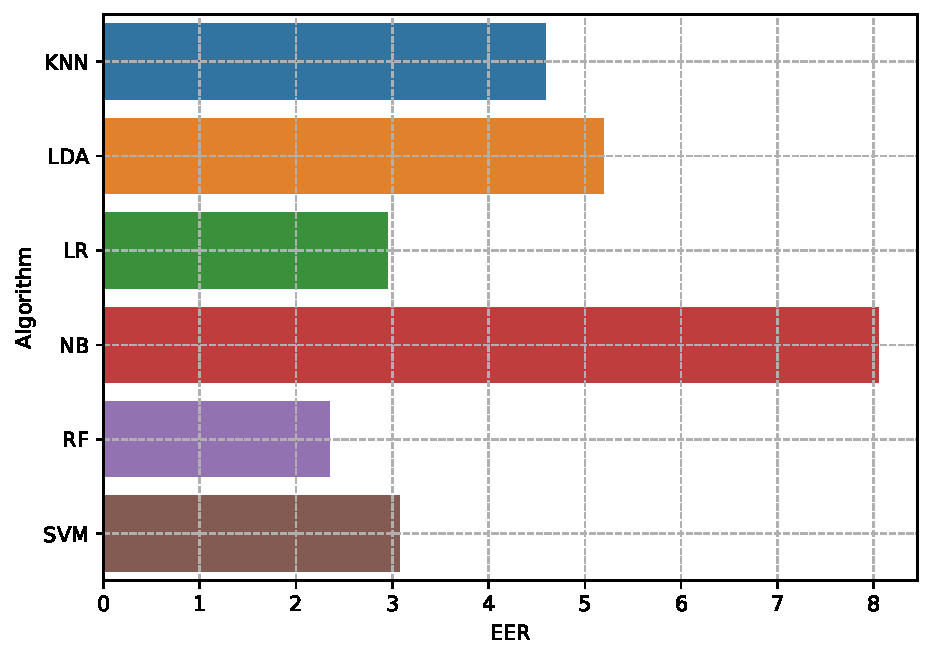
\includegraphics[width=7.60cm]{figures/Results/Other_Plots/Feature_Extraction/ERPCORE/ERPCORE_PSD.pdf}}}%
    \qquad
    \subfloat[\centering Effect of PSD features on the performance of the dataset Mantegna2019]{{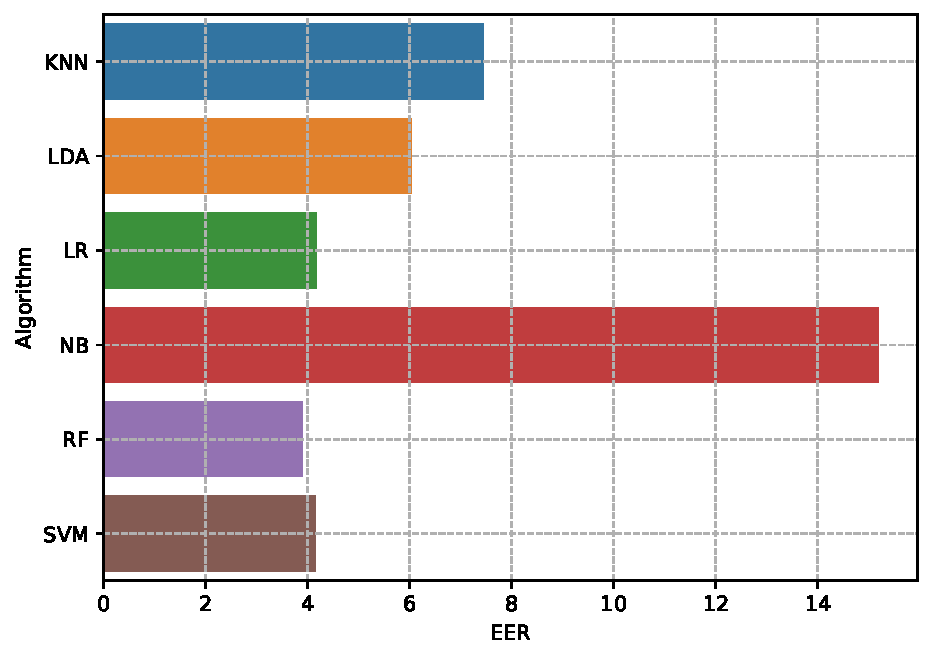
\includegraphics[width=7.6cm]{figures/Results/Other_Plots/Feature_Extraction/MANTEGNA/MANTEGNA_PSD.pdf}}}%
    
     \caption{Impact of Power Spectral Density (PSD) Features on the performance of the datasets. Figures (a), (b), (c) and (d) depicts the change in the EER of the traditional classifiers for the datasets BrainInvaders51a, COG-BCI Flanker, ERPCORE: N400 and Mantegna2019 respectively.}%
    
    \label{fig: Feature Extraction using PSD}%
\end{figure}

%%%%%%%%%%%%%%%%%%%%%%%%%%%%%%%%%%%%%%%%%%%%%%%%%%%%%%%%%%%%%%%%%%%%%
%%%%%%%%%%%%%%%%%%%%%%%%% AR+PSD Features %%%%%%%%%%%%%%%%%%%%%%%%%%%
%%%%%%%%%%%%%%%%%%%%%%%%%%%%%%%%%%%%%%%%%%%%%%%%%%%%%%%%%%%%%%%%%%%%%
\begin{figure}%
    \centering
    \subfloat[\centering Effect of the combination of AR (from order 1 to 10) and PSD features on the performance of the dataset BrainInvaders15a]{{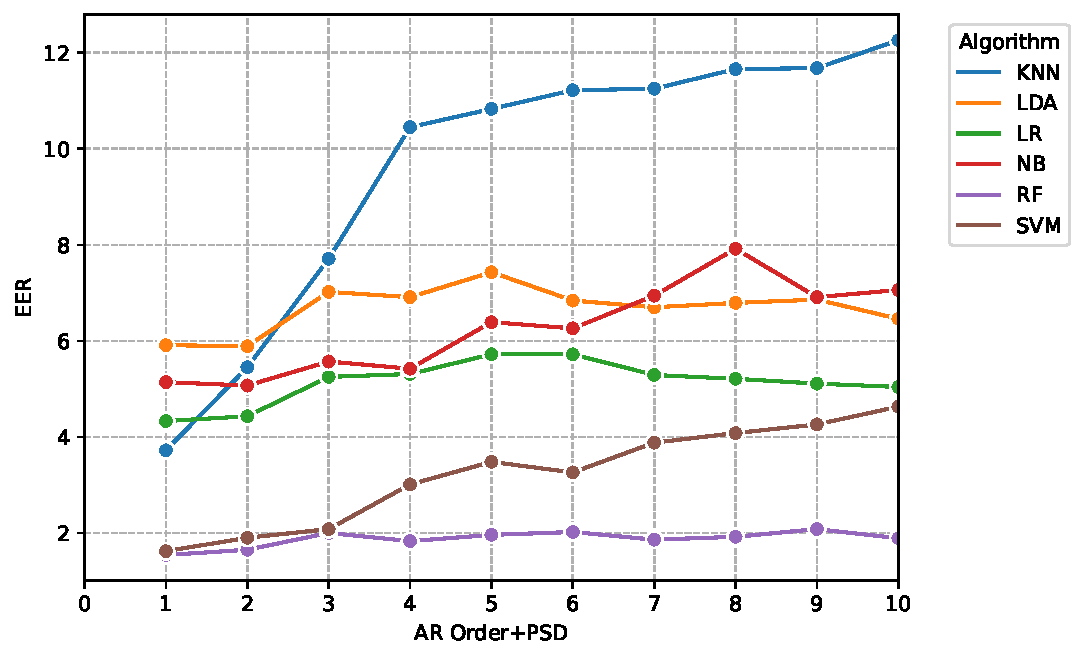
\includegraphics[width=7.60cm]{figures/Results/Other_Plots/Feature_Extraction/BrainInvaders/Brain_AR_PSD.pdf}}}%
    \qquad
    \subfloat[\centering Effect of the combination of AR (from order 1 to 10) and PSD features on the performance of the dataset COG-BCI Flanker]{{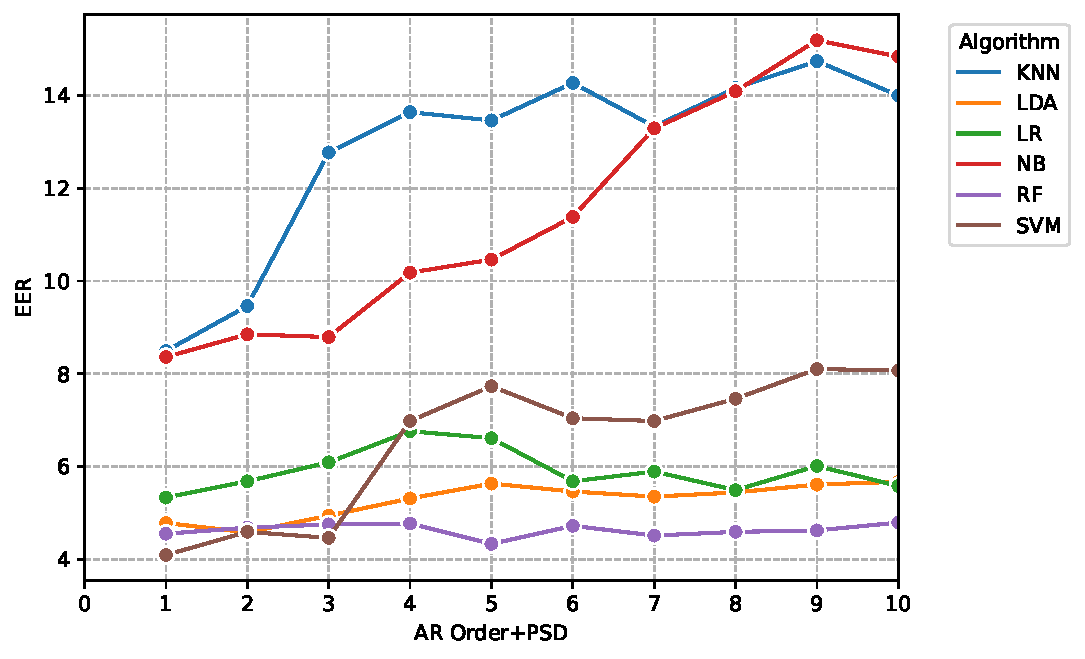
\includegraphics[width=7.60cm]{figures/Results/Other_Plots/Feature_Extraction/COGBCI/cog_AR_PSD.pdf}}}%
    
    
     \subfloat[\centering Effect of the combination of AR (from order 1 to 10) and PSD features on the performance of the dataset ERPCORE: N400]{{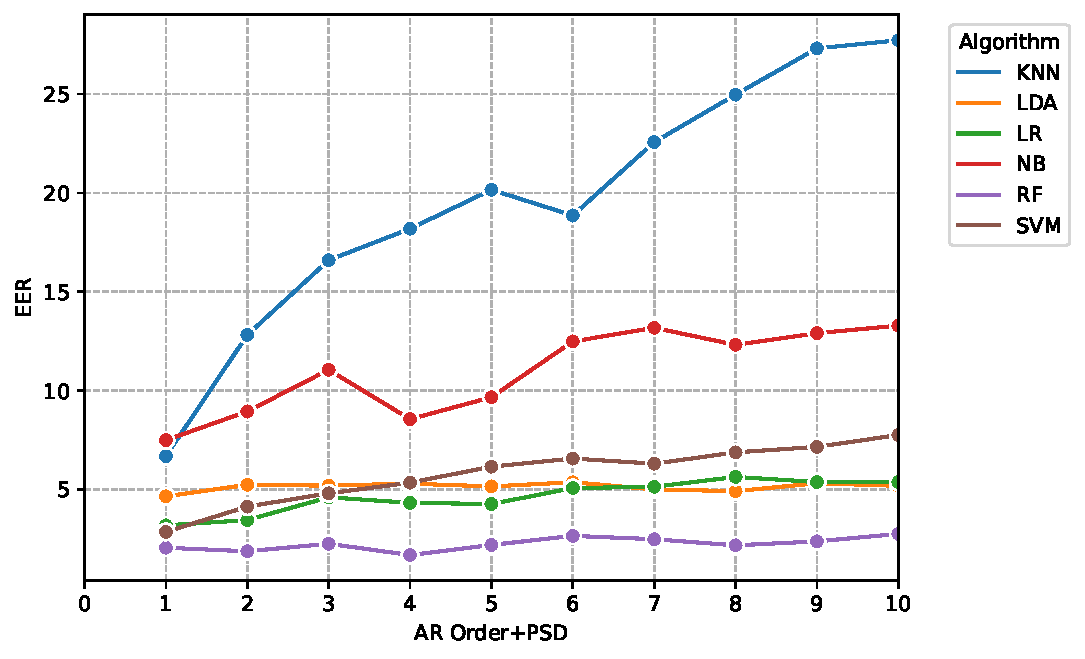
\includegraphics[width=7.60cm]{figures/Results/Other_Plots/Feature_Extraction/ERPCORE/ERPCORE_AR_PSD.pdf}}}%
    \qquad
    \subfloat[\centering Effect of the combination of AR (from order 1 to 10) and PSD features on the performance of the dataset Mategna2019]{{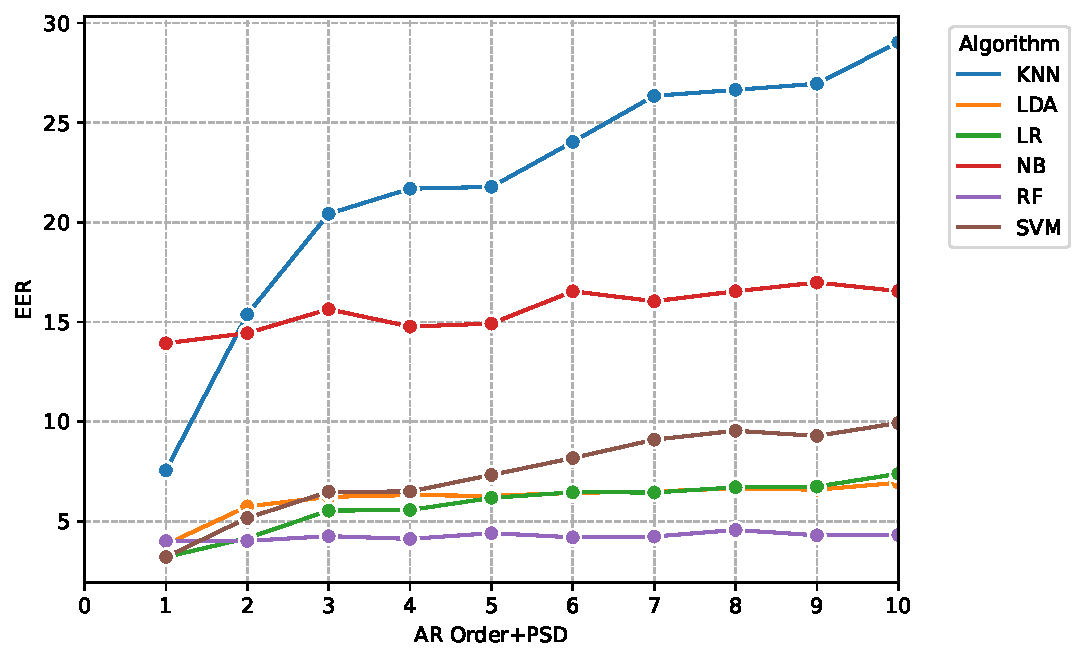
\includegraphics[width=7.6cm]{figures/Results/Other_Plots/Feature_Extraction/MANTEGNA/MANTEGNA_AR_PSD.pdf}}}%
    % \caption{Impact of Auto Regressive(AR) Features with orders from 1 to 10 on the performance of the dataset.}%
    \caption{The influence of combining PSD and AR features with orders ranging from 1 to 10 is assessed in terms of the datasets' performance. The corresponding changes in the EER of traditional classifiers for the BrainInvaders51a, COG-BCI Flanker, ERPCORE: N400, and Mantegna2019 datasets are illustrated in Figures (a), (b), (c), and (d) respectively.}%
    \label{fig: Feature Extraction using AR and PSD}%
\end{figure}
\subsection{Impact of Feature Extraction on Performance}
Feature extraction plays a crucial role in developing a resilient EEG-based authentication system. In this section, we will assess the impact of different feature extraction steps on the performance of all datasets. In our study, we extracted features in the time domain by estimating the AR coefficients and in the frequency domain by calculating Power Spectral Density. These features were passed as input to the classifiers for training and testing. Siamese Networks can acquire discriminant patterns from time series epochs data, as described in Section \ref{sec:Framework:Classification:Similarity Based Learning}.
Consequently, their performance is independent of the AR and PSD features. Accordingly, this section will evaluate the efficacy of traditional classifiers on the four datasets. For each dataset, we extracted 17 unique feature sets (10 AR, 1 PSD, and 10 combinations of both AR and PSD) and evaluated their classification performance. These feature sets included AR coefficients (order=1,2,3,4,5,6,7,8,9,10) of the epoch, PSD of the epoch, and a combination of the two. 
\smallskip

Figure \ref{fig: Feature Extraction using AR} portrays the performance of traditional classifiers on the four datasets, showcasing the impact of varied AR orders. The optimal performance is evident for the BrainInvaders15a, ERPCORE: N400, and Mantegna2019 datasets when employing the lowest AR order, 1. Remarkably, the analyzed datasets demonstrate an increase in EER as the AR order increases. Notably, the COG-BCI Flanker dataset exhibits an EER increase from orders 1 to 3, followed by a consistent decline from orders 3 to 10. However, the data presented underscores a noticeable improvement in classifier efficiency at an AR order of 6. The LDA classifier emerges with the lowest EER across varying AR orders among the classifiers tested.
\smallskip

As depicted in Figure \ref{fig: Feature Extraction using PSD}, the classifiers' performance utilizing only PSD features outperforms that evaluated through AR features. The data in Figure \ref{fig: Feature Extraction using PSD} indicates that the EER remains below 16$\%$ across all classifiers and datasets. Conversely, the utilization of AR features, as shown in Figure \ref{fig: Feature Extraction using AR}, results in a notably higher EER, reaching up to 45$\%$ for the KNN classifier on datasets like ERPCORE: N400 and Mantegna2019. This observation indicates that frequency domain features capture distinct EEG patterns across subjects more effectively than time domain features. It is noteworthy that, once again, the RF classifier stands out as the best performer. 
\smallskip

While the performance of the classifiers improved using PSD features, the best performance across all datasets is achieved using a combination of AR and PSD features, as depicted in \ref{fig: Feature Extraction using AR and PSD}. This observation highlights the significant benefits of incorporating both separate and complementary features of EEG signal representation. The integration of temporal dynamics collected by AR features and the frequency-specific information provided by PSD features enhances the robustness and comprehensiveness of the authentication systems. This integration offers classifiers with a broader and more varied range of characteristics, which is crucial for understanding the intricacies present in EEG signals among various subjects, sessions, and tasks.
%By incorporating these aspects, classifiers can utilize a broader and more varied range of characteristics, which are crucial for interpreting the intricacies of EEG signals in various subjects, sessions, and activities. 

\subsection{Effect on Performance due to Epochs Rejection}
\label{sec:Evaluation:Results:Effect due to different sample size}
The sample size of the dataset passed to the model for learning plays a crucial role in impacting the overall performance of the authentication system. As previously mentioned in section \ref{sec:Framework:Pre-Processing}, the artefact rejection process involves the utilisation of the peak to peak rejection approach. The observation was made that varying rejection thresholds have an impact on the quantity of the dataset that triggers an alert. Consequently, this section will evaluate the influence of various rejection criteria on the efficacy of the best performing traditional classifier, namely RF, as well as the deep learning approach known as Siamese Networks. The evaluation will be performed on the four datasets using the within-session evaluation scheme within the context of the close-set scenario.
\smallskip

% \begin{figure*}
%     %
%     \centering
%      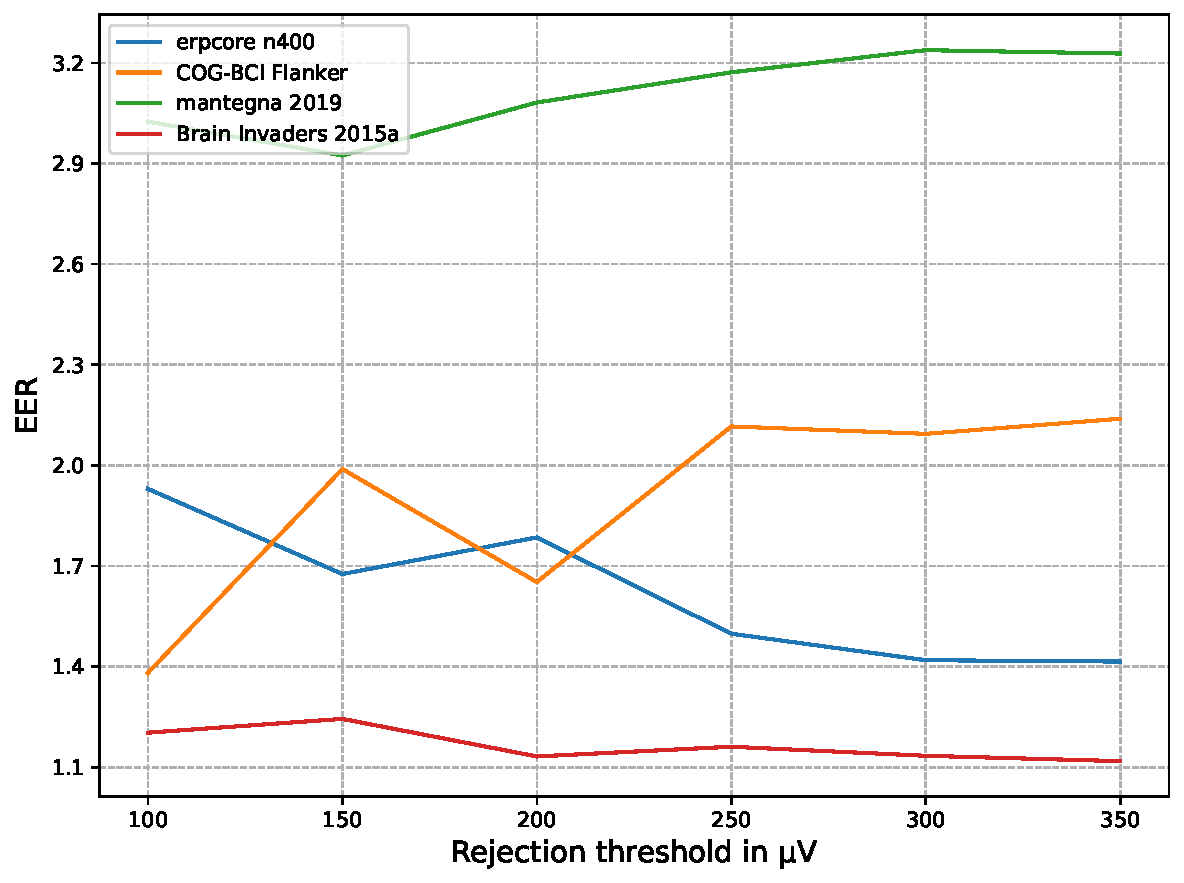
\includegraphics[width=0.75\textwidth]{figures/Results/Other_Plots/Sample_Size/RF_EER.pdf}  
%     %
    
%     %\caption{SMC Learning Algorithm}
%     \caption{Impact of the rejection of epochs on the equal error rate (EER) when using the random forest (RF) classifier is examined across four datasets.}
%     \label{fig: sample_size_RF_EER_Close_set}
% \end{figure*}

\begin{figure}%
    \centering
    \subfloat[\centering Effect of rejection thresholds on EER with RF classification]{{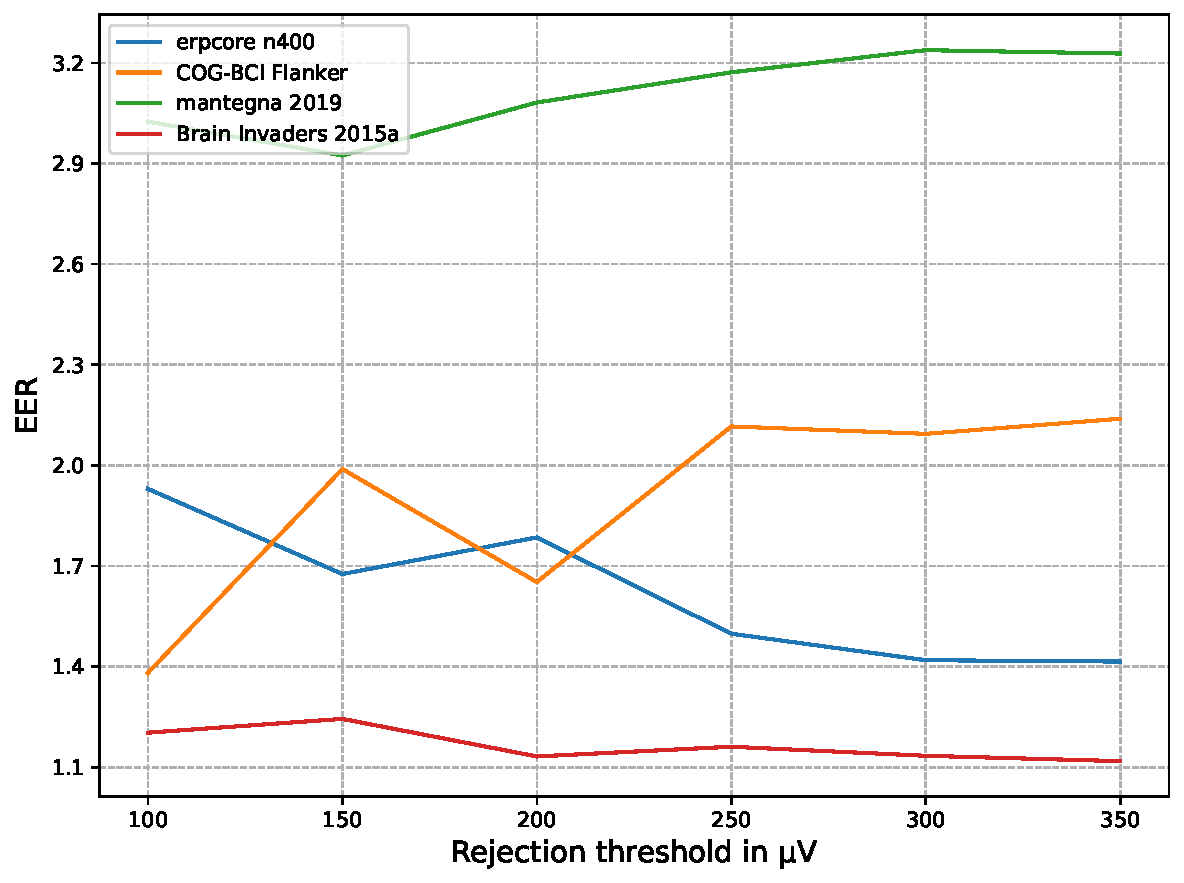
\includegraphics[width=7.5cm]{figures/Results/Other_Plots/Sample_Size/RF_EER.pdf}}}%
    \qquad
    \subfloat[\centering Effect of rejection thresholds on FRR at 1\% FAR with RF classification]{{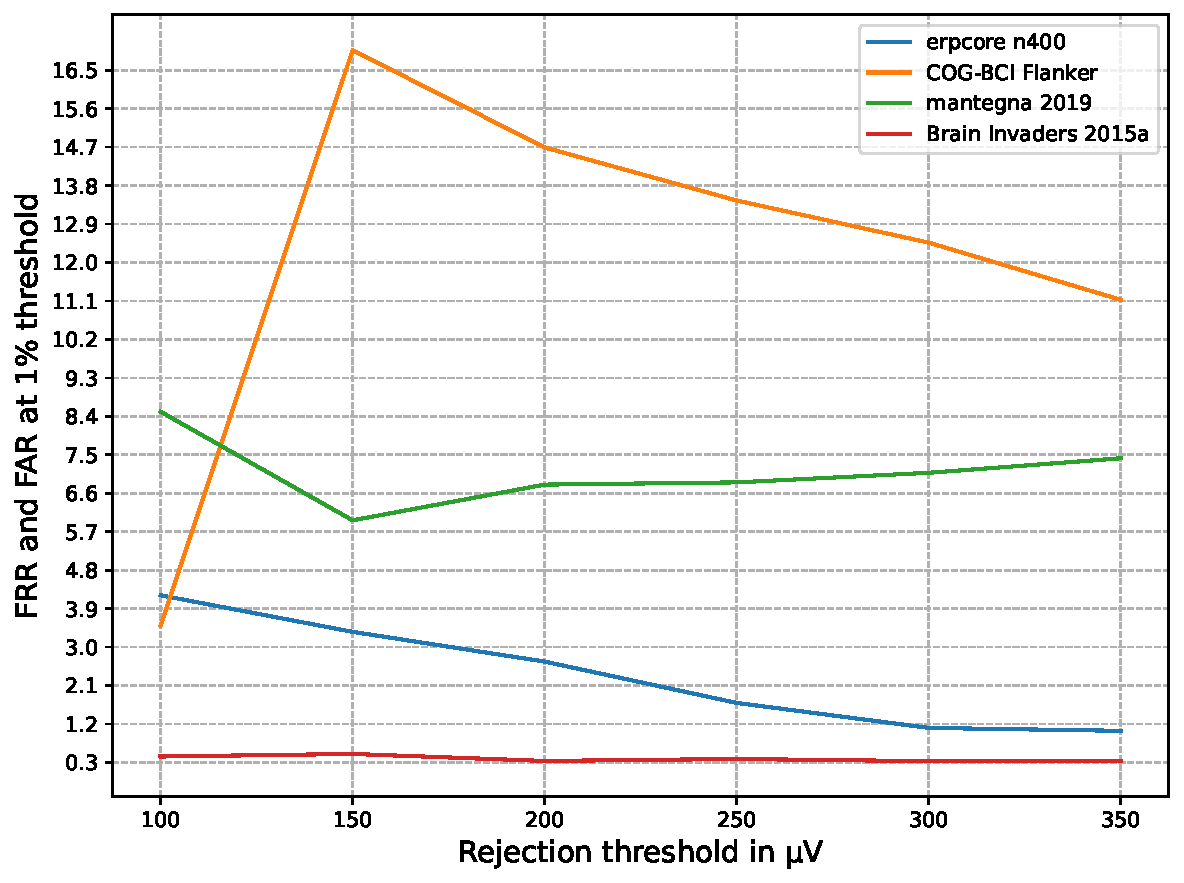
\includegraphics[width=7.5cm]{figures/Results/Other_Plots/Sample_Size/RF_FRR_at_FAR.pdf} }}%
    \caption{Impact of applying epochs rejection on the performance of the four datasets. Figure 6.6 shows the EER and FRR at 1\% FAR for classifier RF.}%
    \label{fig: Effect of sample size}%
\end{figure}

Figure \ref{fig: Effect of sample size} (a) and (b) presents the obtained EER and FRR at 1$\%$ FAR with different rejection thresholds. The results indicate a drop in the EER for the ERPCORE: N400 dataset as the rejection threshold increased from 100$\mu$V to 150$\mu$V. There was a modest increase in EER at 200$\mu$V, followed by a continuous decrease in the EER from 200$\mu$V to 350$\mu$V thresholds. Conversely, a constant reduction in FRR at a FAR of 1$\%$ was observed as the rejection threshold increased from 100$\mu$V to 150$\mu$V. This suggests a positive correlation between the number of samples and the classifier's performance on ERPCORE: N400, indicating that as the number of samples increases, the classifier's performance improves.
Nevertheless, this assumption is not universally applicable to all datasets. In the case of the Mantegna2019 dataset, we noticed a notable increase in the EER as the rejection threshold was raised from 150$\mu$V to 350$\mu$V. However, a slight improvement was observed at the 150$\mu$V threshold, where the EER decreased by 3.66$\%$ (from 3.02$\%$ to 2.92$\%$) and FRR at 1$\%$ FAR drops by 29.84$\%$ (from 8.51$\%$ to 5.97$\%$). This implies that the overall performance of the Mantegna2019 dataset deteriorated as the sample size increased. As the thresholds governing the rejection of epochs are raised, we observe a consistent pattern of improvement and decline in the performance of the RF classifier across the ERPCORE: N400 and Mantegna2019 datasets. However, the COG-BCI Flanker dataset exhibits a distinct pattern in the version of the EER metric, displaying a continuous fluctuation as the thresholds are incrementally increased. Furthermore, it is noteworthy that the dataset BrainInvaders15a demonstrates a minimal shift in EER and FRR at 1$\%$ FAR despite variations in the thresholds for epochs rejection. This observation underlines the dataset's robustness to changes in the rejection threshold, suggesting a consistent performance of the classifier under different rejection conditions.  
%In addition, a minimal change in EER is found for the dataset BrainInvaders15a. 
\smallskip

%From the results shown before, we have to acknowledge that the establishment of a predetermined rejection threshold may impose constraints on the applicability of our methodology, as the magnitude of EEG datasets can differ among different headsets.
Based on the findings mentioned above, it is crucial to recognize that implementing a predetermined threshold for rejection may introduce limitations to the suitability of our methodology, given the size of EEG datasets can vary among different types of headsets and and experimental conditions.
In order to enhance the flexibility of our framework, we have devised a design that allows researchers the choice to specify their own threshold for rejecting epochs. This approach allows for increased customization and adaptation to the unique characteristics of different experimental setups and datasets, thereby enhancing the applicability and robustness of the approach in diverse EEG authentication scenarios.

%However, for this study, we chose 200$\mu$V, and our findings will be reported using this threshold in the section \ref{sec:Evaluation:Results}. 
%refsec:Evaluation:Results.   

%As discussed in section \ref{sec:Framework:Pre-Processing} where we perform artifact rejection using peak to peak rejection method. We highlighted the fact that different rejection thresholds lead to alerting the size of the dataset. 
%As a result, in this section, we will assess the impact of different rejection thresholds on the performance of the best performing traditional classifier i.e., RF and Siamese Networks on the four datasets.       
%The sample size of the dataset passed to the model for learning plays a crucial role in impacting the overall performance of the authentication system. Typically, a larger sample size offers the model a more extensive array of instances, hence facilitating its ability to encompass a wider spectrum of differences in the EEG signals exhibited by various users. Moreover, employing a substantial sample size serves to alleviate the potential issue of overfitting, wherein the model becomes excessively specialised to the training data and encounters difficulties in accurately generalising to unseen data.   
\subsection{Effect on Performance due to Epoch Duration}
\begin{figure}%
    \centering
    \subfloat[\centering Effect of epochs duration on EER with RF classification]{{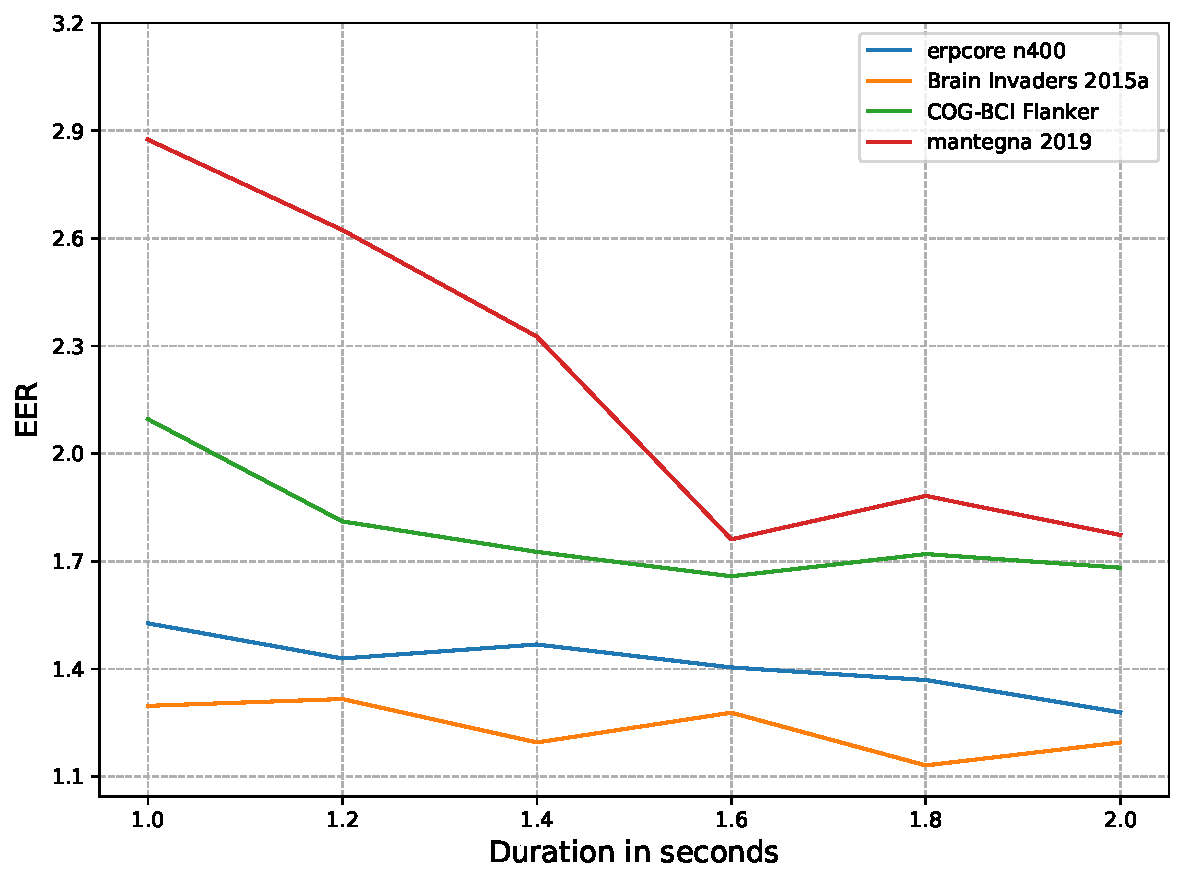
\includegraphics[width=7.55cm]{figures/Results/Other_Plots/Epochs_duration/RF_EER_Epochs_duration.pdf}}}%
    \qquad
    \subfloat[\centering Effect of epochs duration on FRR at 1\% FAR with RF classification]{{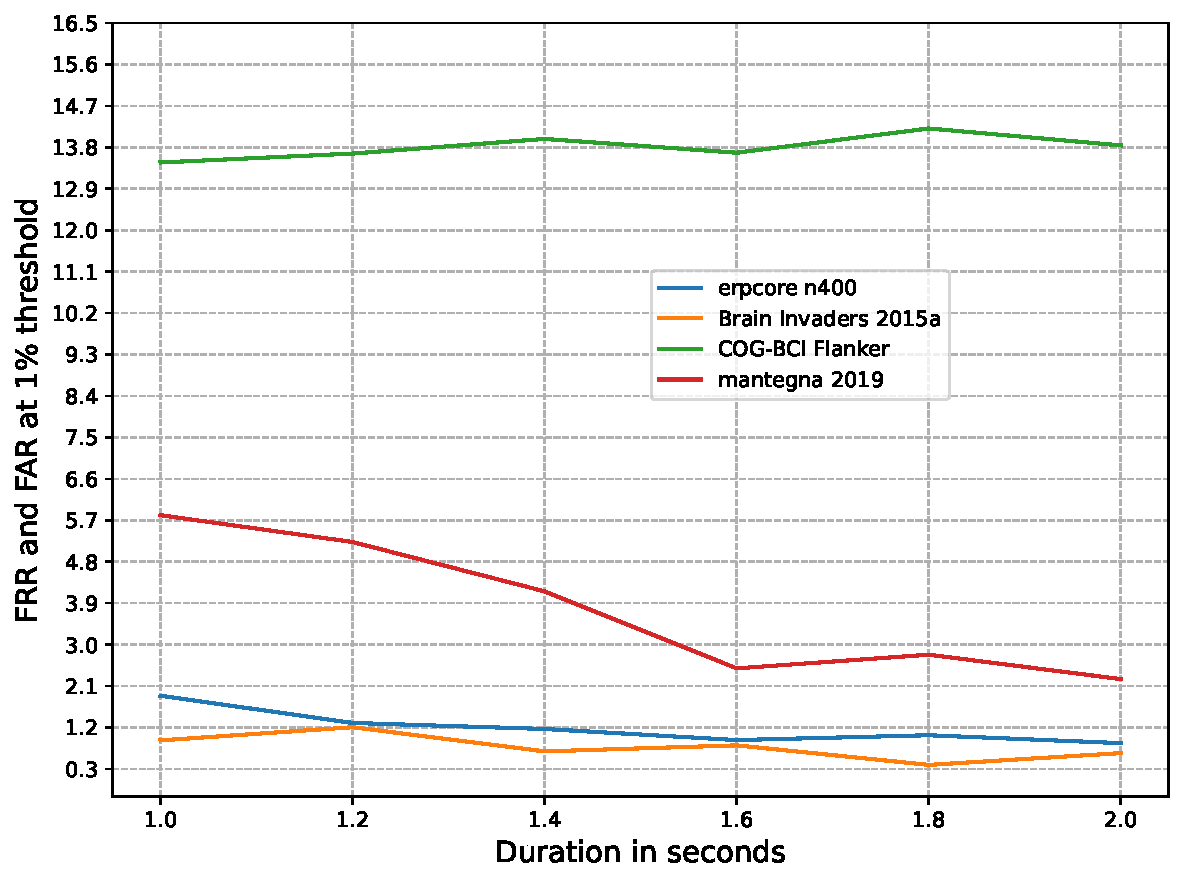
\includegraphics[width=7.55cm]{figures/Results/Other_Plots/Epochs_duration/RF_FRR_1_FAR_Epochs_duration.pdf} }}%
    \caption{Impact of epoch duration on classification scores and epoch rejection on the four datasets. Figure 6.6 shows the EER and FRR at 1\% FAR for classifier RF.}%
    \label{fig: Effect of Epochs Duration}%
\end{figure}
In this section, we analyze the effect of different epochs duration on the performance of our authentication system using RF classifier and same pre-processing and feature extraction pipeline. The durations of the epochs were meticulously arranged, encompassing a range of 1.0 seconds, 1.2 seconds, 1.4 seconds, 1.6 seconds, 1.8 seconds, and 2.0 seconds. Each epoch was preceded by a 200-millisecond interval before the ERP event. The selection of this specific time intervals enables us to thoroughly investigate the impact of various temporal windows surrounding the ERP occurrence on the system's classification performance. Through examining several epochs, our objective is to get vital knowledge regarding the ideal duration that effectively enhances the accuracy and resilience of the authentication system in real world scenario. 
%The epochs were configured to have durations of 1.0, 1.2, 1.4, 1.6, 1.8, and 2.0 seconds, with a starting time of 200 milliseconds before the ERP event. 
\smallskip

As shown in Figure \ref{fig: Effect of Epochs Duration} (a) and (b), the duration of epoch affects the performance of the classifier RF. The figure  illustrates a discernible trend wherein an extension in the epoch duration from 1 second to 2 seconds correlates with a substantial reduction in EER and FRR at 1$\%$ FAR, particularly evident in the case of Mantegna2019 dataset. Notably, for the Mantegna2019 dataset, the EER experiences a noteworthy drop of 38.74$\%$ (from 2.87$\%$ to 1.76$\%$) and the FRR at $\%$ also witnesses a significant decline of 57.24$\%$ (from 5.81$\%$ to 2.48$\%$) as the epochs duration increases from 1 to 1.6 seconds. %There was consistent variation in the EER of dataset BrainInvaders15a as the duration of epochs are increased. The EER increases and decreases with very 0.2 seconds in the epochs length.
The dataset BrainInvaders15a displayed consistent fluctuations in its EER as the epochs' duration was extended. Notably, the EER exhibited oscillations of both increments and decrements, occurring within intervals as short as 0.2 seconds in epochs length.
A marginal alteration in performance is noted for the ERPCORE: N400 and COG-BCI Flanker datasets, as evidenced by the nearly consistent EER and FRR values at a 1$\%$ FAR over increasing epochs duration. 
In contrast, ERPCORE: N400 and COG-BCI Flanker datasets exhibit only marginal shifts in performance. This is evidenced by the nearly unchanging EER and FRR values at 1$\%$ FAR as epochs duration increases.
\smallskip

The variability in datasets performance resulting from varied epoch durations highlights the importance of adaptability within our system. Acknowledging the heterogeneous characteristics of EEG data obtained from various types of headsets and experimental configurations, we have developed our framework to allow the user to customize epoch durations. The option to adjust the duration of epochs will enable researchers to customize the time intervals to align with the unique attributes of their data, hence augmenting the flexibility and resilience of our authentication system.
     

